En esta sección se presentarán diversos artículos de investigación o tesis las cuales abordarán diversas técnicas y enfoques que se emplearon para afrontar problemas similares al de esta tesis. Asimismo, a continuación se presenta un cuadro resumen (véase Anexo \ref{A:table}) de lo que se presenta en esta sección.


\subsection{The Health ChatBots in Telemedicine: Intelligent Dialog System for Remote Support \citep*{HealthChatBots-2022}}
	\subsubsection{Planteamiento del Problema}
		En la actualidad, la implementación de tecnologías avanzadas como el Internet de las Cosas (IoT), Big Data y la inteligencia artificial (IA) en el sector de la salud es esencial para mejorar los servicios de telemedicina. Sin embargo, la interacción tradicional entre pacientes y el sistema de salud carece de herramientas eficientes para la recolección y análisis de datos de salud de manera amigable y precisa. Los métodos convencionales de recopilación de síntomas y datos de pacientes son a menudo tediosos y propensos a errores, lo que puede llevar a diagnósticos imprecisos y a una experiencia de usuario deficiente.
		
		El uso de ChatBots en telemedicina presenta una oportunidad para transformar estas interacciones, permitiendo a los pacientes comunicar sus síntomas y recibir diagnósticos preliminares de manera más interactiva y accesible. No obstante, la implementación de un sistema de ChatBot eficaz enfrenta desafíos significativos, incluyendo la necesidad de una adecuada comprensión del lenguaje natural (NLP), la integración segura de datos de pacientes, y la creación de modelos de aprendizaje automático (ML) precisos y fiables para la predicción de enfermedades
	
	\subsubsection{Objetivos}
		\begin{enumerate}
			\item Desarrollar una plataforma de ChatBot de salud que utilice tecnologías de NLP para mejorar la interacción entre los pacientes y el sistema de salud.\vspace{-2mm}
			\item Implementar modelos de IA y ML para la clasificación y predicción de enfermedades basadas en los síntomas reportados por los pacientes.\vspace{-2mm}
			\item Facilitar la accesibilidad y usabilidad del sistema mediante interfaces de usuario intuitivas y compatibles con el lenguaje natural.\vspace{-2mm}
		\end{enumerate}
			
	\subsubsection{Fundamento Teórico}
		La utilización de ChatBots en el ámbito de la salud se basa en tecnologías avanzadas de NLP y ML para entender y procesar el lenguaje natural de los pacientes. El NLP permite a las máquinas interpretar, analizar y responder a textos generados por humanos. Este proceso incluye diversas técnicas como la lematización, la segmentación morfológica y el etiquetado de partes del discurso, que ayudan a descomponer y entender el texto de entrada.
		
		Los ChatBots de IA están diseñados para imitar la conversación humana utilizando algoritmos de NLP, permitiendo así la recolección de síntomas y la provisión de recomendaciones de autocuidado. Estos sistemas son capaces de analizar grandes volúmenes de datos generados por los usuarios, clasificarlos y extraer insights valiosos mediante algoritmos de ML.
		
		La arquitectura modular del Health Bot, por ejemplo, facilita la escalabilidad y la adaptabilidad del sistema, permitiendo su implementación en diversos escenarios de telemedicina.

	\subsubsection{Metodología empleada por los autores}	
		\begin{figure}[H]
		\begin{center}
			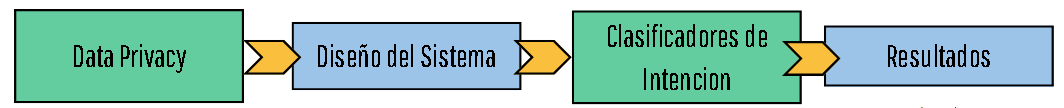
\includegraphics[width=0.8\textwidth]{2/1_antecedentes/Metodologia-1.png}
			\caption{Metodologia. Fuente: \cite{Medbot-2020} }
		\end{center}
	\end{figure}
	\vspace{-10mm}
		\begin{itemize}			
				\item \textbf{Privacidad de Datos}
				Los datos del paciente son protegidos mediante algoritmos de encriptación asimétrica RSA/ECB/PKCS1PADDING. La clave privada RSA es protegida y solo accesible por la capa interna de la API hospitalaria. El Health Bot utiliza la clave pública para desencriptar las solicitudes, garantizando la seguridad de los datos .
		
				\item \textbf{Escalabilidad y Disponibilidad}
				Para asegurar la disponibilidad y escalabilidad de la plataforma, se ha implementado una arquitectura distribuida sin puntos únicos de falla, utilizando servicios de Google Cloud como funciones de Firebase, bases de datos y hosting, BigQuery ML y AI Cloud .
		
					\begin{figure}[H]
						\begin{center}
							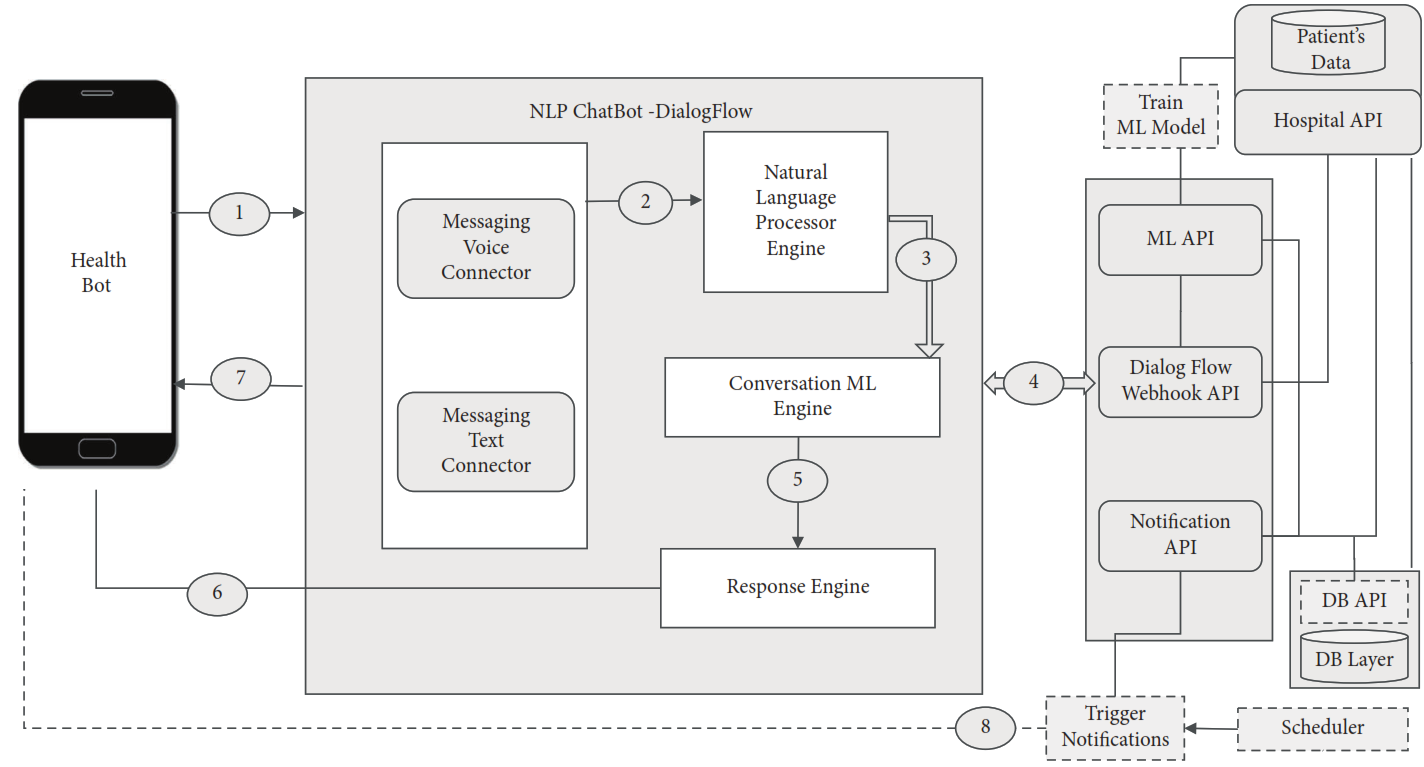
\includegraphics[width=0.7\textwidth]{2/1_antecedentes/Escalabilidad y Disponibilidad.png}
							\caption{Escalabilidad y Disponibilidad. Fuente: \cite{HealthChatBots-2022}}
						\end{center}
					\end{figure}
				\vspace{-10mm}
				\item \textbf{Interfaz de Usuario y Procesamiento NLP}
				El Health Bot UI soporta interfaces conversacionales basadas en texto y voz, desarrollado como una aplicación web progresiva (PWA) para proporcionar una experiencia de usuario nativa. El procesamiento NLP de DialogFlow clasifica las solicitudes de los pacientes y gestiona las respuestas utilizando un flujo de diálogo estructurado .
		
				\begin{figure}[H]
					\begin{center}
						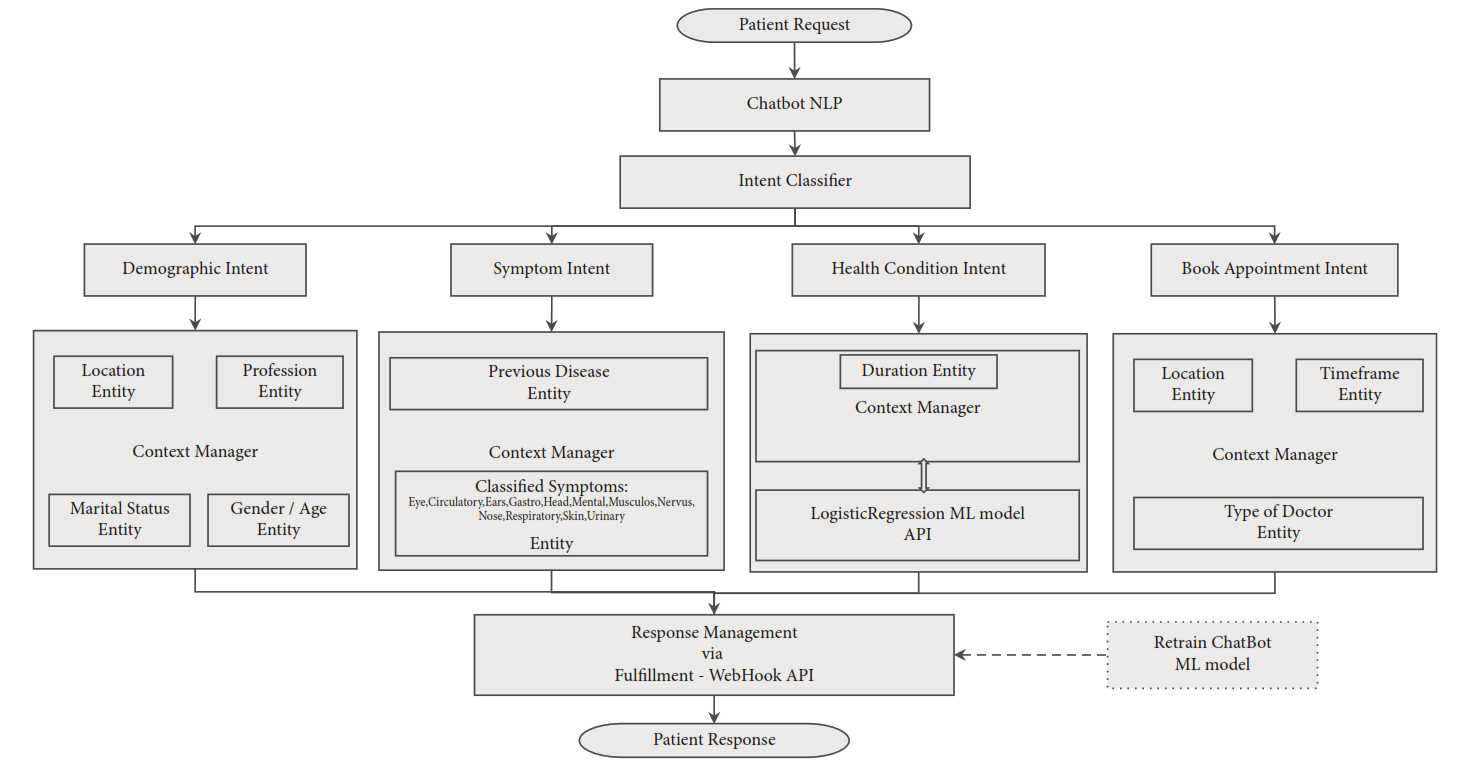
\includegraphics[width=0.7\textwidth]{2/1_antecedentes/Interfaz de Usuario y Procesamiento NLP.png}
						\caption{Interfaz de Usuario y Procesamiento NLP. Fuente: \cite{HealthChatBots-2022} }
					\end{center}
				\end{figure}
		\vspace{-10mm}
				\item \textbf{Clasificadores de Intención} 
				Los clasificadores de intención son responsables de identificar y manejar las preguntas demográficas del paciente, los síntomas conocidos, el estado actual de salud y la programación de citas. Cada intención se gestiona a través de un flujo de contexto que asegura la recogida precisa de datos y la respuesta adecuada del sistema.
		\end{itemize}
			
	\subsubsection{Resultados obtenidos}
	Los resultados del estudio muestran que el Health Bot es capaz de predecir con alta precisión casos de Covid-19 y enfermedades cardíacas. Los modelos de ML entrenados lograron precisiones del 98.3\% y 82\%, respectivamente. En el caso del modelo de Covid-19, se utilizó un conjunto de datos emulado con 2100 filas, de las cuales el 80\% se empleó para entrenamiento y el 20\% para pruebas. El modelo de regresión logística utilizado para predecir enfermedades cardíacas fue entrenado con el conjunto de datos de Cleveland de UCI, logrando un rendimiento del 82\% en precisión.
	
	La implementación de algoritmos de ML y la integración de tecnologías de NLP permitieron una interacción más fluida y precisa entre los pacientes y el sistema de salud, mejorando así la experiencia del usuario y la eficiencia del diagnóstico
	
	\begin{figure}[H]
		\begin{center}
			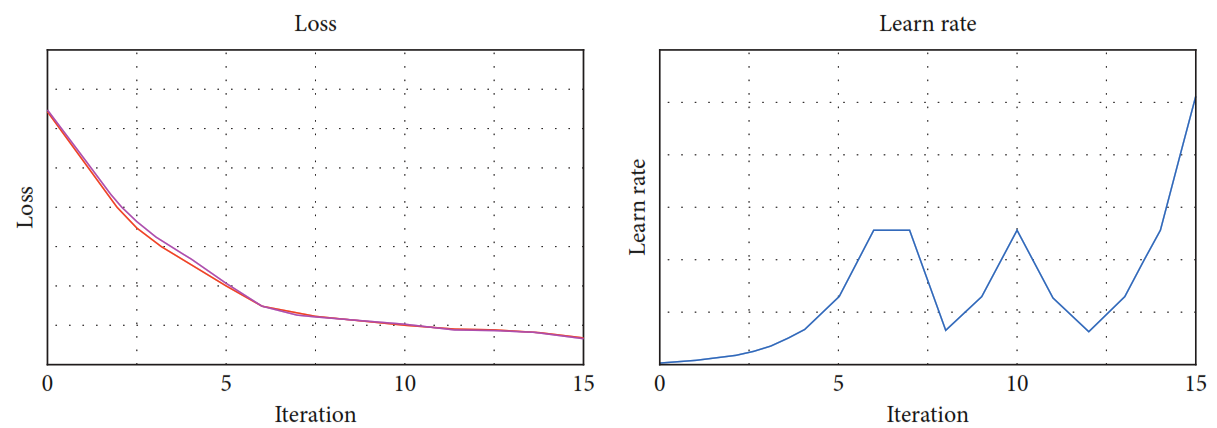
\includegraphics[width=0.8\textwidth]{2/1_antecedentes/Resultado1-1.png}
		\caption{Resultado. Fuente: \cite{HealthChatBots-2022} }
	\end{center}
	\end{figure}
	\vspace{-10mm}
	\begin{figure}[H]
		\begin{center}
			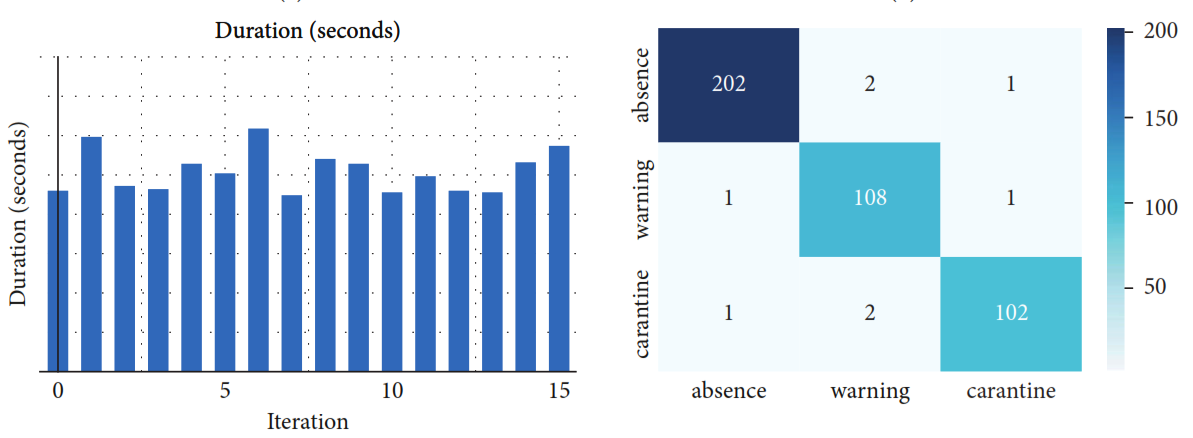
\includegraphics[width=0.8\textwidth]{2/1_antecedentes/Resultado2-1.png}
		\caption{Resultado. Fuente: \cite{HealthChatBots-2022} }
	\end{center}
	\end{figure}
	\vspace{-10mm}
	\begin{figure}[H]
		\begin{center}
			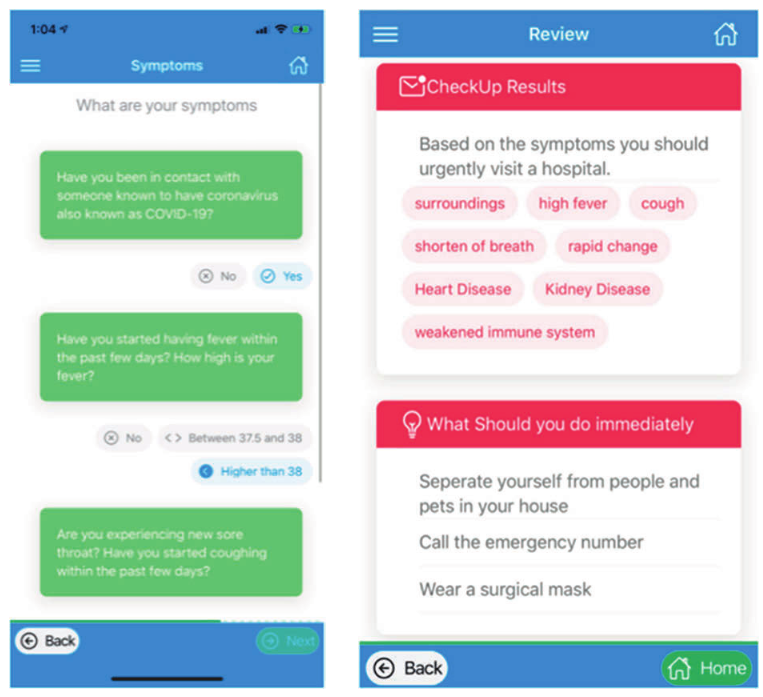
\includegraphics[width=0.7\textwidth]{2/1_antecedentes/Resultado3-1.png}
		\caption{Resultado. Fuente: \cite{HealthChatBots-2022} }
	\end{center}
	\end{figure}
	\vspace{-10mm}
\subsection{PEFT-MedAware: Large Language Model for Medical Awareness \citep*{peftmedaware_2023}}
 %\citep*{pr_dehghani2018copper}}
%\citeauthor{pr_dehghani2018copper} realizaron un artículo de investigación el cual fue publicado en la revista «Resources Policy» en el año 2018. Este fue titulado \citetitle{pr_dehghani2018copper} la cual traducida al español significa «Estimación del precio del cobre utilizando el algoritmo bat».
		\subsubsection{Planteamiento del Problema}
				El artículo "PEFT-MedAware: Large Language Model for Medical Awareness" de Keivalya Pandya aborda el desarrollo de un modelo de lenguaje especializado en la conciencia médica utilizando un enfoque de ajuste fino eficiente en parámetros (PEFT). El problema principal identificado es la inexactitud y la incertidumbre en las respuestas de los modelos de chat generalistas en el ámbito médico, donde la precisión y la fiabilidad son esenciales. Para abordar este problema, se propone un modelo específico, peft-MedAware, que utiliza PEFT para mejorar el modelo Falcon-1b con datos de MedQuAD, que contiene 16,407 pares de preguntas y respuestas médicas. Este enfoque optimiza el rendimiento del modelo utilizando solo el 0.44\% de sus parámetros entrenables, mejorando así la eficiencia computacional. El modelo resultante supera a otros LLMs en tareas de preguntas y respuestas médicas específicas, utilizando recursos computacionales limitados, lo que lo hace adecuado para su implementación en entornos con restricciones de recursos.
		
	\subsubsection{Objetivos}
		\begin{enumerate}
			\item Desarrollar y optimizar el modelo peft-MedAware utilizando técnicas de PEFT para mejorar la precisión en la respuesta a consultas médicas específicas.\vspace{-2mm}		
			\item Aumentar la eficiencia en el entrenamiento de modelos mediante la utilización de configuraciones avanzadas de quantización.\vspace{-2mm}
			\item Proporcionar respuestas médicas contextualmente relevantes y basadas en evidencia a partir de un amplio conjunto de datos médicos.\vspace{-2mm}
		\end{enumerate}
				
	\subsubsection{Fundamento Teórico}
		El fundamento teórico del artículo se basa en el uso de tecnologías avanzadas de procesamiento del lenguaje natural (NLP) y ajuste fino eficiente en parámetros (PEFT) para mejorar la precisión y eficiencia de los modelos de lenguaje en el ámbito médico.
	
		\begin{itemize}
			
			\item \textbf{Procesamiento del Lenguaje Natural (NLP)}
			Se utiliza para analizar y clasificar datos médicos en texto, permitiendo al modelo peft-MedAware proporcionar respuestas precisas y contextualmente relevantes a consultas médicas.
			
			\item \textbf{Ajuste Fino Eficiente en Parámetros (PEFT)}
			El PEFT es una técnica de optimización que ajusta solo los parámetros más influyentes de un modelo, lo que reduce significativamente la sobrecarga computacional y el tiempo de entrenamiento. Esta técnica es crucial cuando se trabaja con grandes modelos de lenguaje, ya que permite un uso más eficiente de los recursos computacionales.
			
			\item \textbf{Modelos de Lenguaje Grande (LLMs)}
			Los LLMs son modelos de inteligencia artificial que contienen miles de millones de parámetros y están diseñados para comprender y generar texto. Estos modelos tienen el potencial de revolucionar la búsqueda de información en el ámbito médico al proporcionar información precisa y actualizada. Sin embargo, su eficacia depende de su capacidad para ofrecer respuestas detalladas y específicas a consultas médicas.
			
				\item \textbf{Quantización}
			La configuración de BitsAndBytes se utiliza para procesar datos y actualizar pesos de manera eficiente durante el entrenamiento de transformadores. La quantización reduce la precisión de los datos procesados, lo que disminuye el consumo de memoria y permite manejar modelos más grandes o múltiples modelos simultáneamente sin sobrecargar los recursos del sistema.
			
				\item \textbf{Datasets Especializados}
			MedQuAD es un conjunto de datos de preguntas y respuestas médicas utilizado para entrenar el modelo peft-MedAware. Este dataset incluye pares de preguntas y respuestas sobre una amplia variedad de enfermedades, medicamentos y otras entidades médicas, proporcionando una base sólida para el entrenamiento y la evaluación del modelo en tareas específicas de QA médico.
		
		\end{itemize}


\subsubsection{Metodología empleada por los autores}
	La metodología utilizada en el desarrollo del modelo peft-MedAware incluye varias etapas críticas, desde la preprocesamiento de datos hasta la implementación de técnicas de ajuste fino y cuantificación para optimizar el rendimiento del modelo.
			\begin{figure}[H]
			\begin{center}
				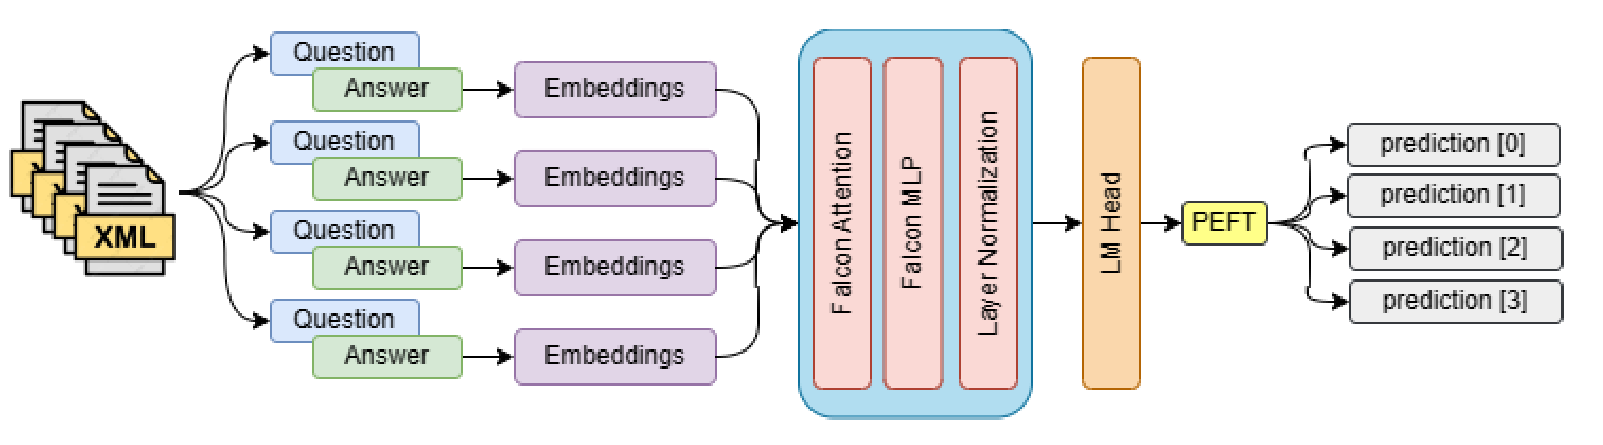
\includegraphics[width=0.8\textwidth]{2/1_antecedentes/Metodologia1- 2.png}
			\caption{Metodologia. Fuente: \cite{peftmedaware_2023}}
			\end{center}
			\end{figure}
			\vspace{-10mm}
		\begin{enumerate}
			\item \textbf{Selección y Preprocesamiento de Datos:}
			
				\subitem \textbf{Dataset MedQuAD:} Se utilizó el conjunto de datos MedQuAD, que contiene 16,407 pares de preguntas y 	respuestas médicas, para entrenar el modelo. Este dataset está bien anotado y cubre una amplia variedad de tipos de preguntas relacionadas con enfermedades, tratamientos, diagnósticos y efectos secundarios.
				
				\subitem \textbf{Preprocesamiento:} Se llevó a cabo un preprocesamiento exhaustivo de los datos para transformar las 	preguntas y respuestas en un formato adecuado para el entrenamiento del modelo. Esto incluye la limpieza de datos, normalización y etiquetado de entidades.
			
			\item \textbf{Entrenamiento del Modelo:}
			
				\subitem \textbf{Ajuste Fino Eficiente en Parámetros (PEFT):} Se aplicó PEFT para ajustar finamente el modelo Falcon-1b utilizando solo el 0.44\% de sus parámetros entrenables (aproximadamente 3 millones de 700 millones). Con esto se redujo la sobrecarga computacional.
			
				\subitem \textbf{Quantización:} Se utilizó la configuración de BitsAndBytes para procesar los datos con precisión de 4 bits, lo que redujo el consumo de memoria y permitió un entrenamiento más eficiente en hardware diverso. Además, se empleó la técnica de doble quantización para capturar características intrincadas de los datos sin comprometer la precisión numérica.
			
			\item \textbf{Configuración del Modelo:}
			
				\subitem \textbf{Carga del Modelo:} El modelo se cargó utilizando precisión de 4 bits, lo que permitió manejar grandes volúmenes de datos y entrenar el modelo de manera eficiente en Google Colab T4 Runtime.
		
				\subitem \textbf{Optimización de Recursos:} La reducción de la complejidad computacional permitió entrenar el modelo más rápidamente y conservar recursos, facilitando la experimentación con varios hiperparámetros y configuraciones sin sobrecargar el sistema.
			
			\item \textbf{Evaluación y Comparación:}
			
				\subitem \textbf{Comparación con Otros Modelos:} Se comparó el rendimiento del modelo peft-MedAware con otros modelos de lenguaje a gran escala, como ChatGPT y Baize-healthcare, en tareas de preguntas y respuestas médicas. 
		\end{enumerate}
		
		\subsubsection{Resultados obtenidos}
			Los resultados del estudio muestran que el modelo peft-MedAware supera a otros modelos de lenguaje en tareas de preguntas y respuestas médicas específicas, utilizando recursos computacionales limitados. El modelo fue capaz de proporcionar respuestas precisas y contextualmente relevantes a una amplia gama de consultas médicas, demostrando una alta eficiencia y especialización. Además, la reducción en los requisitos computacionales permitió tiempos de entrenamiento más rápidos y una mejor eficiencia general del modelo. La implementación de técnicas de PEFT y cuantificación optimizada resultó en un modelo que es tanto preciso como eficiente, adecuado para su despliegue en entornos con restricciones de recursos.

\subsection{Medbot: Conversational Artificial Intelligence Powered Chatbot for Delivering Tele-Health after COVID-19 \citep*{Medbot-2020}} 

		\subsubsection{Planteamiento del Problema}
		La pandemia de COVID-19 ha exacerbado los desafíos existentes en la atención médica, particularmente en áreas rurales de India, donde el acceso a servicios de salud es limitado. El artículo aborda la necesidad de una solución innovadora para superar estas barreras mediante el uso de inteligencia artificial (IA) y tecnologías de telemedicina. Específicamente, propone el desarrollo de un chatbot conversacional multilingüe llamado "Aapka Chikitsak", diseñado para proporcionar educación sanitaria primaria, asesoramiento y medidas preventivas a los pacientes sin necesidad de visitar físicamente un hospital. Este enfoque no solo busca reducir la transmisión del virus, sino también mejorar la accesibilidad y la calidad de la atención médica en un contexto de recursos limitados.
		
	\subsubsection{Objetivos}
		\begin{enumerate}
			\item Aliviar la presión sobre los servicios de salud presenciales mediante la provisión de consultas virtuales.\vspace{-2mm}
			\item Ofrecer información sanitaria básica, medidas preventivas y remedios caseros para enfermedades prevalentes.\vspace{-2mm}
			\item Utilizar procesamiento de lenguaje natural y arquitectura sin servidor para crear un sistema eficiente y escalable.\vspace{-2mm}
			\end{enumerate}
			
	\subsubsection{Fundamento Teórico}
		El fundamento teórico del artículo se basa en varios pilares de la inteligencia artificial y la telemedicina:
		\begin{itemize}
			\item \textbf{Inteligencia Artificial en Salud:} La IA ha demostrado ser eficaz en la simulación de interacciones humanas para proporcionar atención médica. Ejemplos previos incluyen sistemas como ELIZA y PARRY, que imitan interacciones humanas para fines terapéuticos y de diagnóstico.
			\item \textbf{Procesamiento de Lenguaje Natural (NLP):} El uso de NLP permite que los chatbots comprendan y respondan a las consultas de los usuarios en lenguaje natural, facilitando interacciones más humanas y efectivas. Esto incluye la conversión de voz a texto y viceversa, esencial para la funcionalidad del chatbot en múltiples idiomas.
			\item \textbf{Telemedicina:} La telemedicina permite la distribución de servicios de salud a distancia, reduciendo la necesidad de visitas físicas a los centros de salud.
			\item \textbf{Arquitectura sin Servidor:} El (serverless) permite implementar servicios de backend sin necesidad de infraestructura dedicada, lo que facilita la escalabilidad y la eficiencia del sistema.
		\end{itemize}

\subsubsection{Metodología empleada por los autores}
	La metodología empleada en el desarrollo del chatbot $"$Aapka Chikitsak" incluye varios componentes clave:
			\begin{figure}[H]
				\begin{center}
					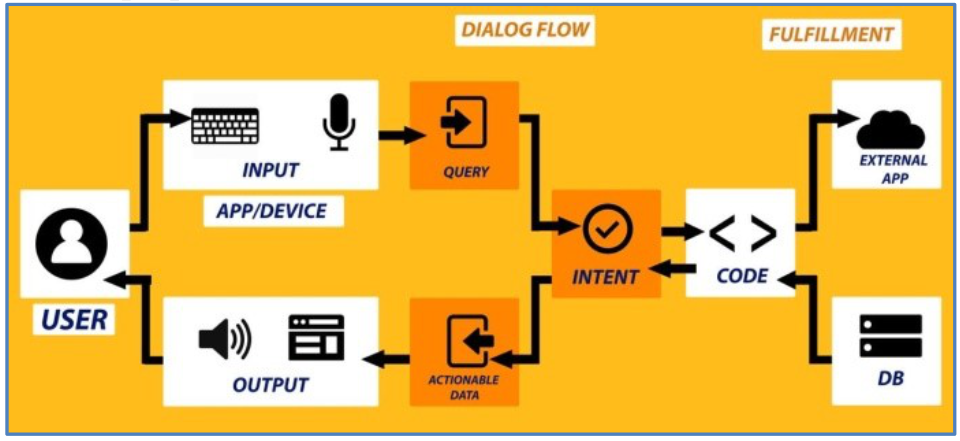
\includegraphics[width=0.6\textwidth]{2/1_antecedentes/Metodologia1- 3.png}
					\caption{Metodologia. Fuente: \cite{Medbot-2020} }
				\end{center}
			\end{figure}
			\vspace{-10mm}
			\begin{enumerate}
	
		\item \textbf{Análisis de Requisitos:} Se identificaron las necesidades de los usuarios, particularmente en áreas rurales, para diseñar un sistema que sea accesible y fácil de usar.
		\item \textbf{Diseño de la Arquitectura:} La aplicación se construyó sobre una arquitectura sin servidor utilizando Google Cloud Platform (GCP) y Firebase Cloud Functions. 
		\item \textbf{Desarrollo del Chatbot:} Se desarrolló un chatbot multilingüe utilizando el API de Dialogflow para la creación de una interfaz conversacional automatizada. El chatbot puede manejar entradas de voz y texto, procesarlas usando NLP y generar respuestas adecuadas.
		\item \textbf{Entrenamiento del Modelo:} Se entrenaron modelos de NLP para reconocer y entender diversas consultas de salud. Los modelos se alimentaron con datos relevantes para mejorar su precisión en la identificación de síntomas y la provisión de consejos médicos.
		\item \textbf{Pruebas y Despliegue:} La aplicación se integró con diversas bases de datos de salud y se sometió a pruebas exhaustivas para asegurar su funcionalidad y precisión. Se realizaron pruebas de usuario para ajustar la interfaz y mejorar la experiencia del usuario. El sistema se desplegó en la infraestructura de GCP, asegurando su disponibilidad y accesibilidad. 
		
	\end{enumerate}
		\subsubsection{Resultados obtenidos}
Los resultados del estudio muestran que el chatbot $"$Aapka Chikitsak" ha logrado reducir significativamente las barreras de acceso a los servicios de salud en las áreas rurales de India. El bot proporciona información sobre las enfermedades más prevalentes, medidas preventivas, remedios caseros y recomendaciones dietéticas basadas en la ubicación del usuario. Además, ofrece sesiones de asesoramiento interactivo para el apoyo emocional y la atención prenatal. La implementación del chatbot ha demostrado ser eficaz en la detección de enfermedades comunes y la provisión de soluciones inmediatas y eficientes a los pacientes.

\subsection{Intelligent Chatbot for Medical Assistance in Rural Areas \citep*{IntelligentChatbot_2020}} 
	\subsubsection{Planteamiento del Problema y objetivo}
		El artículo "Intelligent Chatbot for Medical Assistance in Rural Areas" aborda la problemática de la falta de acceso a servicios médicos en las áreas rurales de la India, donde la mayoría de los doctores y facilidades hospitalarias están concentrados en zonas urbanas. Esto deja a millones de personas sin acceso adecuado a atención médica. Para abordar esta disparidad, los autores han desarrollado una aplicación de chatbot que actúa como un asistente médico virtual, diseñado para conectar a los pacientes rurales con médicos y proporcionar asistencia médica básica. La aplicación utiliza inteligencia artificial para responder consultas médicas, recomendar prácticas de tratamiento y derivar a los pacientes a médicos en casos de problemas más graves. El objetivo es ofrecer una herramienta accesible que pueda brindar información médica esencial, mejorar la autogestión de la salud y reducir la carga sobre los servicios de salud urbanos.
	
	\subsubsection{Fundamento Teórico}
	
	\begin{figure}[H]
		\begin{center}
			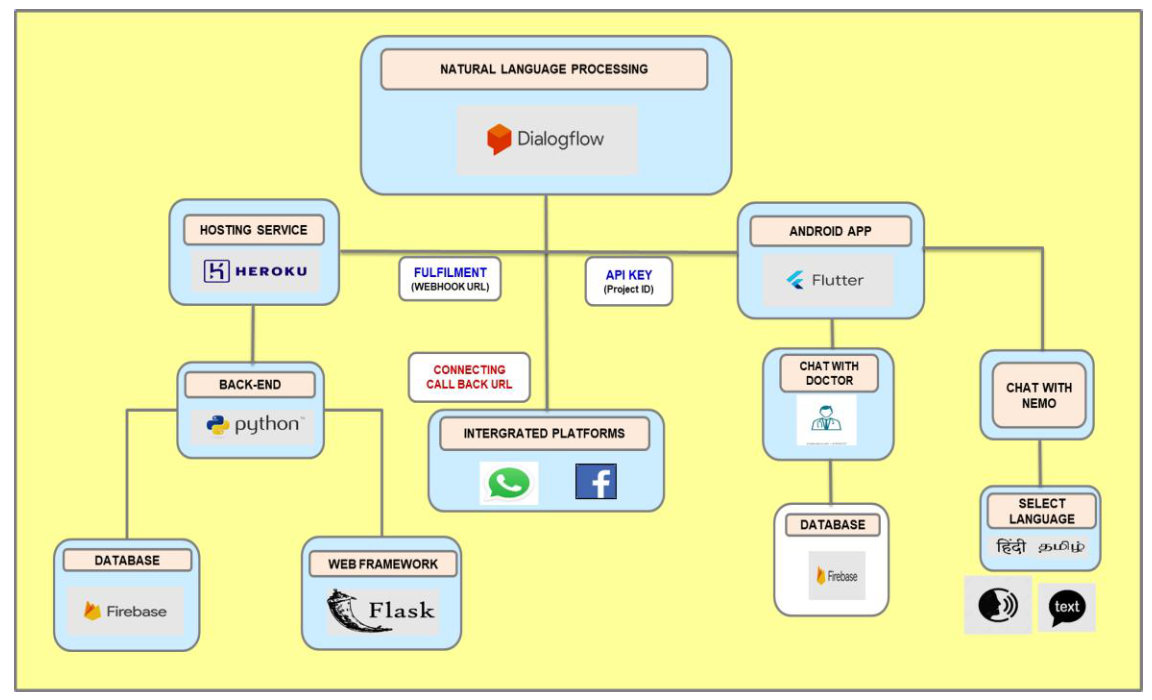
\includegraphics[width=0.8\textwidth]{2/1_antecedentes/Intelligent-FundaTteo.png}
			\caption{Resultado. Fuente: \cite{IntelligentChatbot_2020}}
		\end{center}
	\end{figure}
	\vspace{-10mm}
	
		\begin{itemize}
		\item \textbf{Procesamiento de Lenguaje Natural (NLP):} El NLP permite que los chatbots entiendan y procesen el lenguaje humano. Utilizando algoritmos de NLP, el chatbot puede interpretar las consultas de los usuarios y proporcionar respuestas adecuadas. Esto incluye la identificación de síntomas y la recomendación de tratamientos básicos.
	
		\item \textbf{Arquitectura Sin Servidor:} La aplicación se basa en una arquitectura sin servidor utilizando servicios como Heroku y Firebase. Esto permite una fácil escalabilidad y una gestión eficiente de los recursos, reduciendo la necesidad de infraestructura física.
	
		\item \textbf{Dialogflow:} Esta herramienta se utiliza para desarrollar interfaces conversacionales que soportan la interacción en lenguaje natural. Dialogflow permite la creación de agentes que pueden comprender y responder a las consultas de los usuarios, facilitando una interacción fluida y eficiente.
	
		\item \textbf{Flask y Flutter:} Flask se utiliza como marco web para el desarrollo del backend, mientras que Flutter se emplea para la creación de la interfaz de usuario de la aplicación móvil. Estas herramientas permiten una integración efectiva y una experiencia de usuario intuitiva.
	
		\item \textbf{Algoritmos de Aprendizaje Automático:} Se utilizan algoritmos como Naive Bayes y árboles de decisión para clasificar las consultas de los usuarios y proporcionar respuestas precisas. Estos algoritmos permiten al chatbot aprender y mejorar continuamente a medida que interactúa con más usuarios
		\end{itemize}

	\subsubsection{Metodología empleada por los autores}
	\begin{figure}[H]
		\begin{center}
			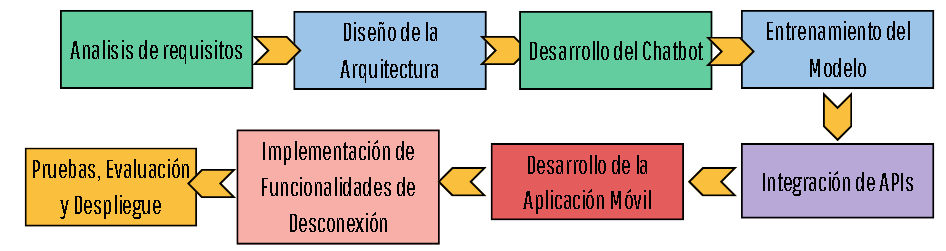
\includegraphics[width=0.8\textwidth]{2/1_antecedentes/Metodologia-4.png}
			\caption{Metodologia. Fuente: \cite{Medbot-2020} }
		\end{center}
	\end{figure}
	\vspace{-10mm}
		\begin{enumerate}
		
		\item \textbf{Análisis de Requisitos:}
		
			\subitem Se realizó un análisis detallado de las necesidades de los usuarios, especialmente en áreas rurales, para diseñar un sistema que sea accesible y fácil de usar.
		
		\item \textbf{Diseño de la Arquitectura:}
		
			\subitem La aplicación se construyó sobre una arquitectura sin servidor utilizando Heroku y Firebase, lo que permite una fácil escalabilidad y reduce la necesidad de infraestructura física.
		
		\item \textbf{Desarrollo del Chatbot:}
			\subitem Se utilizó Dialogflow para crear un agente conversacional que puede manejar entradas de voz y texto. El chatbot utiliza NLP para interpretar las consultas de los usuarios y proporcionar respuestas adecuadas.
	
		\item \textbf{Entrenamiento del Modelo:}
			\subitem Se entrenaron modelos de NLP para reconocer y entender diversas consultas de salud. Estos modelos se alimentaron con datos relevantes para mejorar su precisión en la identificación de síntomas y la provisión de consejos médicos.
			
		\item \textbf{Integración de APIs:}
			\subitem Se integraron varias APIs, como la API de DrugBank para información sobre medicamentos y la API de Practo para datos de médicos. Esto permite al chatbot proporcionar información precisa y relevante sobre tratamientos y profesionales de la salud.
	
		\item \textbf{Desarrollo de la Aplicación Móvil:}
			\subitem Se utilizó Flutter para desarrollar la aplicación móvil, lo que permite una interfaz de usuario intuitiva y una experiencia de usuario fluida. La aplicación está diseñada para ser utilizada en dispositivos Android.
		
		\item \textbf{Implementación de Funcionalidades de Desconexión:}
	
			\subitem Dado que muchas áreas rurales tienen acceso limitado a Internet, se implementaron funcionalidades de comunicación fuera de línea utilizando Twilio. Esto permite a los usuarios interactuar con el chatbot a través de mensajes de texto y llamadas telefónicas, incluso sin una conexión a Internet.
		
		\item \textbf{Pruebas, Evaluación y Despliegue:}
		
			\subitem La aplicación se sometió a pruebas exhaustivas para asegurar su funcionalidad y precisión. Se realizaron pruebas de usuario para ajustar la interfaz y mejorar la experiencia del usuario. Además, se evaluó la precisión de las respuestas del chatbot mediante la comparación con respuestas proporcionadas por profesionales de la salud. El sistema se desplegó en la infraestructura de Heroku y Firebase, asegurando su disponibilidad y accesibilidad
			
		\end{enumerate}

	\subsubsection{Resultados obtenidos}
		Los resultados presentados en el estudio muestran que el chatbot es capaz de proporcionar información médica precisa y útil a los usuarios rurales, mejorando significativamente el acceso a servicios médicos básicos. La aplicación ha sido bien recibida por los usuarios, con una alta tasa de interacción y satisfacción. El análisis de las sesiones de usuario indica que el chatbot maneja eficazmente una variedad de consultas médicas, proporcionando respuestas rápidas y relevantes. Los usuarios han utilizado principalmente el chatbot para consultas sobre síntomas comunes, medicación y recomendaciones de primeros auxilios. Además, la capacidad del chatbot para operar sin conexión constante a internet ha sido un factor crucial en su aceptación y uso en áreas rurales con infraestructura limitada de internet.
	\begin{table}[H]
		\centering
			\begin{tabular}{l|ccc}
				\multicolumn{1}{c|}{INTENT} & \multicolumn{1}{c|}{SESSIONS} & \multicolumn{1}{c|}{COUNT} & \multicolumn{1}{c|}{EXIT\%} \\ \hline
				FIND DOCTOR & 10 & 52 & 1.92 \\
				FIND DOCTOR-CUSTOM & 8 & 48 & 18.75 \\
				SMALLTALK.GREETINGS.HELLO & 6 & 22 & 18.18 \\
				WEATHER & 5 & 16 & 12.50 \\
				FEVER & 4 & 12 & 8.33 \\
				FIND HOSPITAL & 5 & 11 & 2.50 \\
				FIND HOSPITAL-CUSTOM & 4 & 9 & 22.22 \\
				WEATHER-CUSTOM & 2 & 9 & 8.90 \\
				DIABETES & 3 & 7 & 2.10 \\ \hline
			\end{tabular}
		\caption{Resultado. Fuente: \cite{IntelligentChatbot_2020}}
	\end{table}


%\vspace{-10mm}

\subsection{HHH: An Online Medical Chatbot System based on Knowledge Graph and Hierarchical Bi-Directional Attention \citep*{HHHAnOnlineMedical}} %\citep*{pr_dehghani2018copper}}
%\citeauthor{pr_dehghani2018copper} realizaron un artículo de investigación el cual fue publicado en la revista «Resources Policy» en el año 2018. Este fue titulado \citetitle{pr_dehghani2018copper} la cual traducida al español significa «Estimación del precio del cobre utilizando el algoritmo bat».
	\subsubsection{Planteamiento del Problema y objetivo}
		El artículo "HHH: An Online Medical Chatbot System based on Knowledge Graph and Hierarchical Bi-Directional Attention" aborda los problemas que enfrentan los pacientes para acceder a servicios de atención primaria, como la dificultad para ver a un médico, largos tiempos de espera y la inconveniencia de hacer citas. Para abordar estos desafíos, los autores proponen un sistema de chatbot médico que combina un grafo de conocimiento con un modelo de atención bidireccional jerárquico (HBAM). El chatbot, denominado HHH (Healthcare Helper System), está diseñado para responder preguntas médicas complejas utilizando un grafo de conocimiento construido a partir de datos médicos recopilados de Internet y un modelo de similitud de texto basado en aprendizaje profundo. Este enfoque híbrido permite al chatbot comprender y responder preguntas en lenguaje natural, proporcionando respuestas precisas y relevantes a los usuarios con poco conocimiento médico. El objetivo principal es mejorar la eficiencia y calidad del servicio médico, facilitando el acceso a información médica y reduciendo el desperdicio de recursos.

	\subsubsection{Fundamento Teórico}
	El fundamento teórico del trabajo se basa en la combinación de dos enfoques:grafo de conocimiento y HBAM para procesar y responder preguntas en el contexto médico.
		
		\begin{itemize}
			\item \textbf{ Grafo de Conocimiento:} El grafo de conocimiento almacena información médica, incluyendo enfermedades, síntomas, tratamientos y relaciones entre estos conceptos. Este proporciona respuestas rápidas y precisas a preguntas bien definidas, aprovechando la estructura organizada y fácilmente consultable del grafo.
		
			\item \textbf{Modelo de Atención Jerárquico Bidireccional (HBAM):} Este modelo es una extensión de los modelos LSTM (Long Short-Term Memory), que son una clase de redes neuronales recurrentes (RNN) diseñadas para procesar secuencias de datos. El HBAM incluye una capa de BiLSTM que captura información de contexto en ambas direcciones (hacia adelante y hacia atrás) y una capa de atención que resalta las palabras clave en una oración.
		
			\item \textbf{Siamese Framework y Distancia Manhattan:} El modelo utiliza un enfoque de redes siamés, donde dos redes idénticas comparten los mismos pesos para procesar dos entradas diferentes y comparar sus representaciones. La distancia Manhattan se utiliza para medir la similitud semántica entre las representaciones de las oraciones.
		\end{itemize}
		
%El uso combinado de estos enfoques permite al sistema HHH manejar una amplia variedad de preguntas médicas, proporcionando respuestas tanto desde un grafo de conocimiento como utilizando modelos de aprendizaje profundo para comparar y entender la semántica de las consultas en lenguaje natural.

\subsubsection{Metodología empleada por los autores}
La metodología adoptada para el desarrollo del sistema HHH incluye varios componentes y pasos clave para garantizar su efectividad y precisión:

\begin{figure}[H]
	\begin{center}
		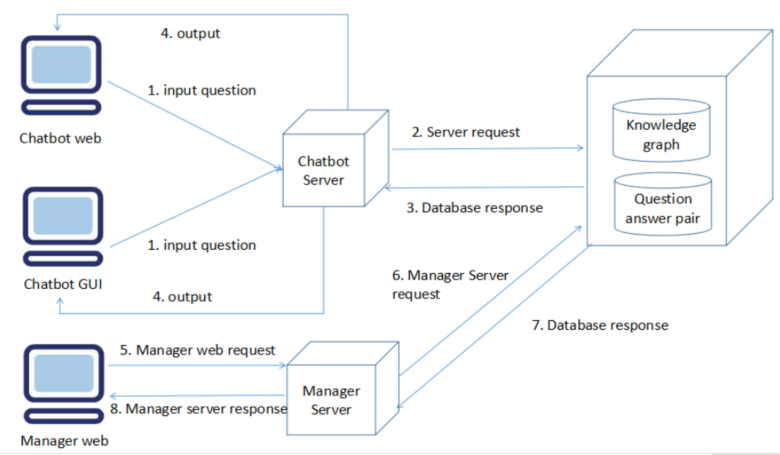
\includegraphics[width=0.6\textwidth]{2/1_antecedentes/Metodologia-5.png}
		\caption{Metodologia. Fuente: \cite{HHHAnOnlineMedical} }
	\end{center}
\end{figure}
\vspace{-10mm}
	\begin{enumerate}
	
		\item \textbf{Diseño de la Arquitectura del Sistema:}
			\subitem \textbf{Arquitectura del Gráfico de Conocimiento:} Se desarrolló utilizando Neo4j, que almacena datos sobre enfermedades, síntomas y tratamientos. El gráfico contiene 3,500 entidades y 4,500 relaciones.
		
			\subitem \textbf{Modelo HBAM:} Incluye una capa de LSTM bidireccional y una capa de atención de palabras, diseñada para comparar la similitud semántica entre preguntas y respuestas en el dataset.
		
		\item \textbf{Implementación del Gráfico de Conocimiento:}
		
			\subitem \textbf{Almacenamiento y Recuperación de Datos:} El gráfico de conocimiento se construyó a partir de datos médicos recopilados de diversas fuentes en línea. El proceso de selección de respuestas implica la extracción de entidades relevantes y la identificación de la intención del usuario.
		
			\subitem \textbf{Extracción de Entidades y Reconocimiento de Intenciones:} Utiliza el algoritmo Aho-Corasick para identificar entidades médicas en las preguntas de los usuarios y un módulo de reconocimiento de intenciones para predecir la intención del usuario basada en bibliotecas de predicados predefinidos.
		
		\item \textbf{Desarrollo del Modelo HBAM:}
		
			\subitem \textbf{Entrenamiento y Pruebas:} El modelo se entrenó utilizando un subconjunto del dataset de preguntas duplicadas de Quora, que contiene pares de preguntas y respuestas médicas. Se utilizó una capa de LSTM bidireccional para capturar la información contextual y una capa de atención para resaltar las palabras clave en las preguntas.
	
			\subitem \textbf{Evaluación del Modelo:} Se comparó el rendimiento del HBAM con otros modelos de vanguardia como BERT y MaLSTM. Los resultados mostraron que HBAM tiene un mejor rendimiento en términos de precisión en la similitud semántica.
		
		\item \textbf{Integración de la Interfaz de Usuario:}
		
			\subitem \textbf{Interfaz Web y GUI Local:} Se desarrollaron para permitir la interacción del usuario con el chatbot. La interfaz web facilita el acceso remoto, mientras que la GUI local proporciona una experiencia de usuario enriquecida.
		
		\item \textbf{Pruebas y Evaluación del Sistema:}
		
			\subitem \textbf{Pruebas de Usuario:} Se realizaron pruebas exhaustivas para asegurar la funcionalidad y precisión del sistema. Los usuarios interactuaron con el chatbot para evaluar la calidad de las respuestas y la facilidad de uso de la interfaz.
		
		\item \textbf{Despliegue y Mantenimiento:}
		
			\subitem \textbf{Implementación en Entornos Reales:} El sistema se desplegó en entornos de producción para evaluar su rendimiento en situaciones reales. Se implementó un sistema de monitoreo continuo para mantener la calidad del servicio y realizar mejoras basadas en el feedback de los usuarios.
		
	\end{enumerate}

	\subsubsection{Resultados obtenidos}
		Los resultados obtenidos muestran que el modelo HBAM supera a otros modelos de última generación en términos de precisión en la predicción de la similitud de oraciones médicas. En los experimentos realizados, el HBAM logró una precisión promedio del 81.2\%, comparado con el 78.2\% de BERT y el 78.4\% de MaLSTM. Estos resultados indican que el HBAM es más efectivo en la comprensión de consultas médicas y la provisión de respuestas precisas.

		Además, el sistema HHH demostró ser capaz de manejar una variedad de preguntas médicas, proporcionando respuestas precisas y relevantes tanto desde el grafo de conocimiento como mediante la comparación de similitud de texto. Los experimentos adicionales realizados con conjuntos de datos médicos adicionales confirmaron la robustez y flexibilidad del modelo HBAM, mostrando un rendimiento consistente en diferentes escenarios de prueba.

		\begin{table}[h!]
			\centering
			\caption{Metodos de comparacion. Fuente:  \cite{HHHAnOnlineMedical}}
			\begin{tabular}{ccc}
				\hline
				\textbf{Methods} & \textbf{Average Evaluation Accuracy} & \textbf{Range of Change by 30 Times Experiments} \\ \hline
				BERT [7] & 78.2\% & (-1.8\%,+1.3\%) \\
				MaLSTM [9] & 78.4\% & (-2.9\%,+2.0\%) \\
				HBAM & 81.2\% & (-2.4\%,+2.2\%) \\
				\hline
			\end{tabular}
		\end{table}
		
		\begin{table}[h]
			\centering
			\begin{tabular}{|>{\raggedright}p{4cm}|>{\raggedright}p{2.5cm}|>{\raggedright}p{3.5cm}|>{\raggedright\arraybackslash}p{4.5cm}|}
				\hline
				\textbf{Medical website name} & \textbf{Method name} & \textbf{Average predict accuracy} & \textbf{Range of change by 10 times experiments} \\
				\hline
				\multirow{3}{*}{ehealthforumQAs} 
				& BERT & 78.5\% & (-1.8\%, +1.1\%) \\
				& HBAM & \textbf{81.3\%} & (-1.2\%, +1.1\%) \\
				& MaLSTM & 78.4\% & (-2.9\%, +1.5\%) \\
				\hline
				\multirow{3}{*}{questionDoctorQAs} 
				& BERT & 78.2\% & (-1.4\%, +0.9\%) \\
				& HBAM & \textbf{80.9\%} & (-2.1\%, +2.5\%) \\
				& MaLSTM & 78.1\% & (-1.7\%, +1.9\%) \\
				\hline
				\multirow{3}{*}{webmdQAs} 
				& BERT & 78.1\% & (-1.6\%, +0.9\%) \\
				& HBAM & \textbf{81.2\%} & (-1.2\%, +1.3\%) \\
				& MaLSTM & 78.5\% & (-1.5\%, +1.9\%) \\
				\hline
			\end{tabular}
			\caption{Resultado de exactitud. Fuente: \cite{HHHAnOnlineMedical}}
		\end{table}

%\vspace{-10mm}

\subsection{HealFavor: Dataset and A Prototype System for Healthcare ChatBot \citep*{HealFavor}} %\citep*{pr_dehghani2018copper}}
%\citeauthor{pr_dehghani2018copper} realizaron un artículo de investigación el cual fue publicado en la revista «Resources Policy» en el año 2018. Este fue titulado \citetitle{pr_dehghani2018copper} la cual traducida al español significa «Estimación del precio del cobre utilizando el algoritmo bat».
	\subsubsection{Planteamiento del Problema}
		El acceso a servicios médicos puede ser difícil debido a varios factores, como la escasez de médicos, largos tiempos de espera y la inconveniencia de hacer citas. Estas barreras afectan tanto a pacientes como a proveedores de servicios de salud, resultando en un uso ineficiente de los recursos disponibles. En respuesta a estos desafíos, se han desarrollado sistemas innovadores como los chatbots médicos basados en inteligencia artificial. Estos sistemas tienen el potencial de simular conversaciones en tiempo real, proporcionando asistencia médica interactiva y personalizada. El trabajo presentado propone el desarrollo de un chatbot médico llamado HealFavor, que utiliza un conjunto de datos autogenerado y una arquitectura prototipo para mejorar la accesibilidad médica y proporcionar respuestas precisas a consultas médicas comunes.

\subsubsection{Fundamento Teórico}
El fundamento teórico del sistema de chatbot HealFavor se basa en la integración de técnicas avanzadas de inteligencia artificial y procesamiento de lenguaje natural (NLP). Estos enfoques permiten al sistema comprender y responder a consultas médicas en lenguaje natural, proporcionando respuestas precisas y relevantes.

\begin{itemize}
	
	\item \textbf{ Sistemas de Chatbot Históricos y Contemporáneos}
		El desarrollo de chatbots se remonta a sistemas pioneros como ELIZA, desarrollado en la década de 1960, que utilizaba patrones de scripts codificados para simular conversaciones. ALICE, que utilizaba patrones basados en el lenguaje de marcado de inteligencia artificial (AIML), mejoró esta capacidad al almacenar respuestas en archivos AIML. Sistemas más recientes como Jabberwacky y Cleverbot no solo utilizan respuestas preprogramadas, sino que también aprenden de las interacciones pasadas para mejorar sus respuestas
	
	\item \textbf{Arquitectura del Sistema:} La aplicación HealFavor se basa en el marco de RASA, utilizando políticas de diálogo embebidas recurrentes para la generación de respuestas. La integración con MongoDB permite el almacenamiento en tiempo real de historiales de chat y análisis de informes médicos, facilitando un sistema escalable y eficiente.
	\end{itemize}
\subsubsection{Metodología empleada por los autores}
La metodología adoptada para el desarrollo del sistema HHH incluye varios componentes y pasos clave para garantizar su efectividad y precisión:
	\begin{figure}[H]
		\begin{center}
			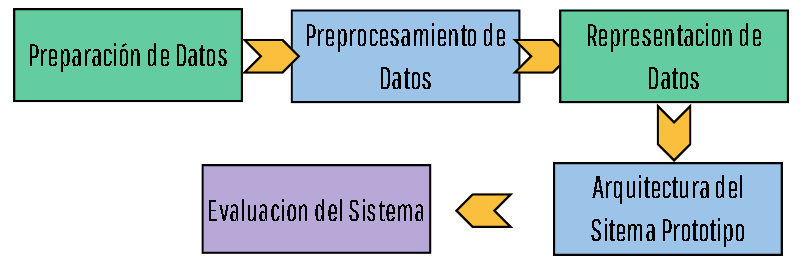
\includegraphics[width=0.8\textwidth]{2/1_antecedentes/Metodologia-6.png}
			\caption{Metodologia. Fuente: \cite{Medbot-2020} }
		\end{center}
	\end{figure}
	\vspace{-10mm}
	\begin{enumerate}
		
		\item \textbf{Preparación de Datos:}
			\subitem \textbf{Fuentes y Observaciones:} Los datos se recopilaron de fuentes confiables como WebMD y Drugs.com, y se consultó con expertos médicos para obtener información sobre síntomas comunes.
			\subitem \textbf{Calidad y Filtrado:} Los datos preparados se verificaron para asegurar su consistencia y relevancia. Se realizaron grandes clasificaciones iniciales para abarcar un amplio conjunto de enfermedades y luego se refinaron según síntomas específicos.
		\item \textbf{Preprocesamiento de Datos:}
			\subitem \textbf{Técnicas Utilizadas:} Incluyen conversión a minúsculas, eliminación de palabras vacías, tokenización y lematización para mejorar la clasificación y precisión de los datos.
		\item \textbf{Representación de Datos:}
			\subitem \textbf{Clasificación de Intenciones:} Se desarrollaron módulos para clasificar las intenciones de los pacientes como un problema de clasificación múltiple. Las secuencias de intenciones se utilizaron para predecir las respuestas y continuar la conversación.
			\subitem \textbf{Predicción de Secuencias:} Se prepararon conjuntos exhaustivos de secuencias para diferentes casos de uso de pacientes, incluyendo preguntas relacionadas con la salud y la reserva de citas.
		\item \textbf{Arquitectura del Sistema Prototipo:}
			\subitem \textbf{Marco RASA:} Utiliza políticas de diálogo embebidas recurrentes inspiradas en el algoritmo StarSpace de Facebook AI Research. Se crean vectores de características utilizando la representación de Bag of Words (BoW) y se generan incrustaciones a través de capas densas para la entrada del paciente y las acciones del sistema.
			\subitem \textbf{Mecanismo de Atención:} El input del usuario y el output previo de la red se alimentan en un modelo recurrente para calcular la atención, utilizando la suma total del output de la capa de incrustación y del mecanismo de atención para generar la respuesta final.
		\item \textbf{Evaluación del Sistema:}
			\subitem \textbf{Pruebas de Usuario:} Se realizaron pruebas exhaustivas con evaluadores que hicieron un total de 162 preguntas al sistema. Las respuestas se calificaron en una escala de 1 a 3, obteniendo una precisión total del 46.50\%.
	\end{enumerate}

\subsubsection{Resultados obtenidos}
	El sistema de chatbot HealFavor ha demostrado ser efectivo en la provisión de respuestas precisas y relevantes a preguntas médicas comunes. Los resultados de las pruebas de usuario mostraron una alta satisfacción con la precisión de las respuestas y la facilidad de uso de la interfaz. El sistema alcanzó una precisión del 46.50\% en la clasificación de respuestas correctas, lo que indica una mejora significativa en la accesibilidad médica y la eficiencia del sistema de salud. La integración con MongoDB permitió el almacenamiento en tiempo real de historiales de chat y análisis de informes médicos, facilitando un sistema escalable y eficiente.

\subsection{ChatDoctor: A Medical Chat Model Fine-Tuned on a Large Language Model Meta-AI (LLaMA) Using Medical Domain Knowledge \citep*{chatdoctor}} 
\subsubsection{Planteamiento del Problema}
	El acceso a consultas médicas precisas y oportunas sigue siendo un desafío significativo, especialmente en regiones con recursos médicos limitados. Los modelos de lenguaje grandes (LLMs) como ChatGPT han demostrado capacidades impresionantes en tareas generales de procesamiento del lenguaje natural (NLP), pero su rendimiento en el dominio médico es limitado debido a la falta de entrenamiento específico en conocimientos médicos. Esto puede resultar en respuestas incorrectas que pueden ser perjudiciales en un contexto médico. Para abordar esta limitación, se desarrolló el modelo ChatDoctor, afinado específicamente en el conocimiento del dominio médico utilizando el modelo LLaMA. Este modelo busca mejorar la precisión y relevancia de las respuestas médicas, proporcionando así un apoyo más fiable y accesible para los pacientes y profesionales de la salud.

\subsubsection{Fundamento Teórico}
El desarrollo de ChatDoctor se basa en varios principios teóricos y tecnológicos clave:

	\begin{itemize}
		\item \textbf{Modelo de Lenguaje Grande (LLM):} Los LLMs como LLaMA se entrenan inicialmente en grandes cantidades de datos textuales para predecir la siguiente palabra en una secuencia, desarrollando así habilidades generales de lenguaje. Estos modelos luego se afinan utilizando conjuntos de datos específicos del dominio para mejorar su rendimiento en tareas especializadas.
		
		\item \textbf{Afine del Modelo con Datos Específicos del Dominio:} ChatDoctor se afina utilizando un conjunto de datos de 100,000 conversaciones médico-paciente reales recopiladas de una plataforma de consulta médica en línea. Este enfoque asegura que el modelo desarrolle una comprensión profunda de las consultas y respuestas médicas auténticas.
		
		\item \textbf{Recuperación Autónoma de Información:} Para mitigar las limitaciones inherentes a los LLMs, como las respuestas erróneas, se incorpora una base de conocimientos externos que el modelo puede consultar en tiempo real. Esta base de conocimientos incluye bases de datos médicas confiables y recursos en línea como Wikipedia. La recuperación de información se realiza a través de prompts configurados que extraen términos clave de las consultas del paciente y buscan la información relevante en la base de conocimientos.
		
		\item \textbf{Evaluación de Rendimiento:} El rendimiento de ChatDoctor se evalúa utilizando métricas estándar como precisión, recuerdo y puntuación F1, comparándolo con otros modelos como ChatGPT. Estas evaluaciones se realizan utilizando respuestas de médicos humanos como referencia para garantizar la relevancia y exactitud de las respuestas generadas por el modelo.
	\end{itemize}

\subsubsection{Metodología empleada por los autores}
	La metodología adoptada para el desarrollo del sistema HHH incluye varios componentes y pasos clave para garantizar su efectividad y precisión:

	\begin{figure}[H]
		\begin{center}
			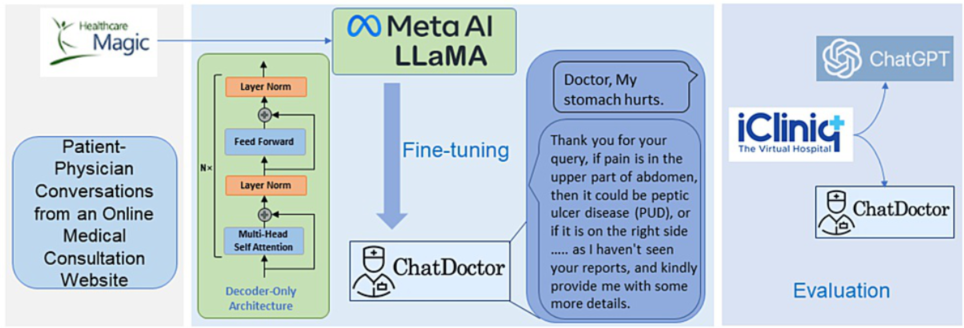
\includegraphics[width=0.8\textwidth]{2/1_antecedentes/Metodologia-7.png}
			\caption{Metodologia del proceso del modelo del ChatDoctor. Fuente: \cite{chatdoctor} }
		\end{center}
	\end{figure}
	\vspace{-10mm}
	\begin{enumerate}
		
		\item \textbf{Recolección y Preparación de Datos:}
			
			\subitem \textbf{Dataset de Conversaciones Médico-Paciente:} Se recopilaron alrededor de 100,000 interacciones médico-paciente de la plataforma HealthCareMagic. Estas conversaciones se limpiaron y anonimizaron para respetar la privacidad de los participantes.
			
			\subitem \textbf{Filtrado de Conversaciones: }Se eliminaron automáticamente las conversaciones demasiado cortas y se filtraron manualmente las respuestas con errores. Se utilizó LanguageTool para corregir errores gramaticales y asegurar la calidad de los datos.
				
			\subitem \textbf{Dataset de Pruebas:} Se recopilaron alrededor de 10,000 conversaciones adicionales de iCliniq para probar el rendimiento del modelo.
			
		\item \textbf{Desarrollo de la Base de Conocimientos Externa:}
			
			\subitem \textbf{Curación de la Base de Datos:} Se creó una base de datos que incluye enfermedades, síntomas, pruebas médicas y tratamientos utilizando fuentes confiables como MedlinePlus. Esta base de datos es actualizable continuamente sin necesidad de reentrenamiento del modelo.
			
			\subitem \textbf{Recuperación de Información:} Se diseñaron prompts específicos para extraer términos clave de las consultas del paciente y buscar información relevante en la base de conocimientos. Este proceso asegura respuestas precisas y respaldadas por fuentes confiables.
		
		\item \textbf{Entrenamiento del Modelo:}
			
			\subitem \textbf{Modelo LLaMA:} Se utilizó el modelo LLaMA de Meta, entrenado en 1.0 billón de tokens de fuentes de datos públicas. Este modelo fue afinado primero con datos del proyecto Alpaca de Stanford y luego con el dataset HealthCareMagic-100k utilizando 6 GPUs A100 durante tres horas.
			
			\subitem \textbf{Parámetros de Entrenamiento:} Los parámetros incluyeron un tamaño de batch total de 192, una tasa de aprendizaje, 3 épocas, una longitud máxima de secuencia de 512 tokens y una proporción de calentamiento de 0.03, sin decaimiento de peso.
		
		\item \textbf{Evaluación del Modelo:}
			
			\subitem \textbf{Pruebas de Rendimiento:} Se utilizaron preguntas del dataset iCliniq como entradas y las respuestas de médicos humanos como referencia. Se empleó BERTScore para evaluar la precisión, el recuerdo y la puntuación F1 de las respuestas generadas por ChatDoctor en comparación con ChatGPT.
			
			\subitem \textbf{Comparaciones Cualitativas:} Se realizaron comparaciones detalladas entre las respuestas de ChatDoctor y ChatGPT en términos de precisión y relevancia para diversas consultas médicas contemporáneas.
	\end{enumerate}

\subsubsection{Resultados obtenidos}
	El modelo ChatDoctor mostró un rendimiento superior en la provisión de respuestas médicas precisas y relevantes en comparación con ChatGPT. En pruebas cualitativas, ChatDoctor fue capaz de responder correctamente a preguntas sobre términos médicos recientes como Monkeypox y medicamentos aprobados recientemente como Daybue, gracias a su capacidad de recuperación autónoma de información. En evaluaciones cuantitativas utilizando BERTScore, ChatDoctor superó a ChatGPT en precisión, recuerdo y puntuación F1, demostrando su efectividad en proporcionar respuestas médicas fiables. Estas mejoras subrayan el potencial de ChatDoctor para asistir en consultas médicas preliminares y mejorar la accesibilidad a la información médica precisa.

		\begin{table}[h!]
			\centering
			\begin{tabular}{|c|c|c|c|}
				\hline
				& \textbf{ChatGPT} & \textbf{ChatDoctor} & \textbf{P-value} \\
				\hline
				\textbf{Precision} & 0.8374 $\pm$ 0.0188 & 0.8444 $\pm$ 0.0185 & $6.66 \times 10^{-19}$ \\
				\hline
				\textbf{Recall}    & 0.8445 $\pm$ 0.0164 & 0.8451 $\pm$ 0.0157 & $4.71 \times 10^{-4}$ \\
				\hline
				\textbf{F1 Score}   & 0.8406 $\pm$ 0.0143 & 0.8446 $\pm$ 0.0138 & $2.14 \times 10^{-111}$ \\
				\hline
			\end{tabular}
			\caption{Comparacion entre el BERTScore entre ChatDoctor y Chatgpt. Fuente: \cite{chatdoctor} }
		%	\label{tabla:metricas}
		\end{table}

%\vspace{-10mm}
\subsection{Auto Response Generation in Online Medical Chat Services \citep*{AutoResponse-2022}}
	\subsubsection{Planteamiento del Problema y objetivo}
	El acceso a servicios médicos de calidad y la eficiencia en la comunicación entre médicos y pacientes son desafíos significativos en el campo de la telemedicina. Con el aumento de la demanda de consultas médicas en línea debido a la pandemia de COVID-19 y otros factores, los profesionales de la salud enfrentan una carga de trabajo elevada que puede afectar la calidad de la atención médica. En respuesta a este problema, el estudio propone un mecanismo de generación de respuestas automáticas inteligentes para servicios de chat médico en línea, con el objetivo de mejorar la eficiencia de las interacciones entre médicos y pacientes y reducir los tiempos de espera. Este mecanismo se basa en algoritmos de aprendizaje automático y procesamiento de lenguaje natural para identificar y generar respuestas adecuadas a las consultas de los pacientes, mejorando así la experiencia general del usuario y la efectividad del servicio de telemedicina.
	
	\subsubsection{Fundamento Teórico}
	El desarrollo del sistema de generación de respuestas automáticas inteligentes se basa en varias tecnologías y teorías clave:
		
		\begin{itemize}
			\item \textbf{Procesamiento de Lenguaje Natural (NLP):} En este estudio, se utilizan técnicas de NLP para analizar y procesar las consultas de los pacientes, permitiendo la generación de respuestas adecuadas basadas en la comprensión del contexto y la semántica del texto.
				
			\item \textbf{	Modelos de Aprendizaje Automático: }Se emplean varios algoritmos de aprendizaje automático, incluyendo BERT, BiLSTM, y XGBoost, para entrenar el sistema con un gran conjunto de datos de conversaciones médicas. Estos modelos aprenden a identificar patrones y generar respuestas basadas en el historial de interacciones médicas.
				
			\item \textbf{	Clustering y Filtrado de Datos:} Se utilizan algoritmos de clustering para agrupar respuestas médicas similares y etiquetar manualmente los datos, creando un conjunto de respuestas prediseñadas que el sistema puede utilizar. Este enfoque asegura que las respuestas generadas sean coherentes y relevantes para las consultas de los pacientes.
				
			\item \textbf{	Evaluación y Mejora Continua:} El rendimiento del sistema se evalúa mediante métricas estándar como precisión, recuerdo y puntuación F1, comparando las respuestas generadas con las respuestas proporcionadas por médicos humanos. Este proceso de evaluación permite identificar áreas de mejora y ajustar los modelos para mejorar la precisión y relevancia de las respuestas.
				
		\end{itemize}

	\subsubsection{Metodología empleada por los autores}
		La metodología empleada para desarrollar el sistema de generación de respuestas automáticas inteligentes incluye varias etapas clave:
		\begin{figure}[H]
			\begin{center}
				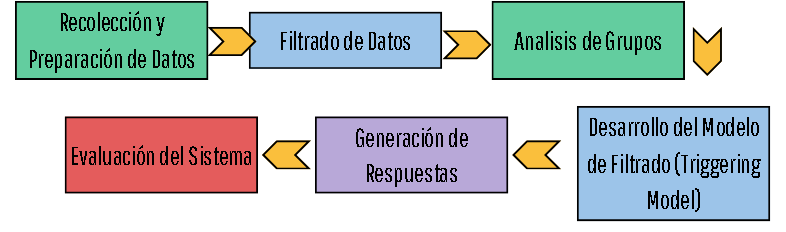
\includegraphics[width=0.6\textwidth]{2/1_antecedentes/Metodologia-8.png}
				\caption{Metodologia. Fuente: \cite{Medbot-2020} }
			\end{center}
		\end{figure}
		\begin{enumerate}
			\vspace{-10mm}
			\item \textbf{Recolección y Preparación de Datos:}
				\subitem \textbf{Dataset de Conversaciones Médico-Paciente:} Se recopilaron más de 900,000 mensajes históricos entre médicos y pacientes a lo largo de 9 meses. Estos datos se anonimizaron y se prepararon para el análisis.
				
				\subitem \textbf{Filtrado de Datos:} Se aplicaron técnicas de limpieza de datos para corregir errores ortográficos, mal uso de puntuación y errores gramaticales, asegurando la calidad del dataset.
			
			\item \textbf{Analisis de Grupos:}
				\subitem \textbf{Clustering de Respuestas Médicas:} Se implementaron algoritmos de clustering para identificar las respuestas más frecuentes de los médicos y etiquetar los datos manualmente. Se crearon clusters semánticos para agrupar respuestas similares y se seleccionaron los clusters más densos para su uso en el sistema.
			
			\item \textbf{Desarrollo del Modelo de Filtrado (Triggering Model):}
			
				\subitem \textbf{Modelo de Clasificación Binaria:} Se desarrolló un modelo de clasificación binaria para filtrar los mensajes de los pacientes y determinar si requieren una respuesta automática. Este modelo se entrenó utilizando técnicas de embedding ponderado y algoritmos como BERT y BiLSTM.
						
			\item \textbf{Generación de Respuestas:}
			
				\subitem \textbf{Modelo de Generación de Respuestas:} Se desarrollaron varios modelos de generación de respuestas, incluyendo BERT y Seq2Seq, para sugerir las respuestas más adecuadas a las consultas de los pacientes que pasaron el filtro de triggering. Estos modelos se entrenaron utilizando el conjunto de datos preprocesado y se ajustaron para maximizar la precisión y relevancia de las respuestas generadas.
			
			\item \textbf{Evaluación del Sistema:}
				\subitem \textbf{Pruebas de Rendimiento:} Se realizaron pruebas exhaustivas para evaluar la precisión, el recuerdo y la puntuación F1 de las respuestas generadas. Se utilizó un enfoque de validación cruzada de 5 pliegues para asegurar la robustez del modelo y evitar el sobreajuste.
				
				\subitem \textbf{Comparación con Baselines:} Se comparó el rendimiento de los modelos desarrollados con enfoques basados en reglas y otros algoritmos de aprendizaje automático, demostrando la efectividad del enfoque propuesto.
		\end{enumerate}
			
\subsubsection{Resultados obtenidos}
	El sistema de generación de respuestas automáticas inteligentes demostró ser altamente efectivo en la provisión de respuestas precisas y relevantes a consultas médicas en línea. Los modelos basados en BERT superaron significativamente a otros algoritmos en términos de precisión y recuerdo, con una precisión@3 de 85.41\%. La integración de técnicas de NLP y aprendizaje automático permitió generar respuestas coherentes y útiles en tiempo real, mejorando la eficiencia de las interacciones médico-paciente. Los resultados indican que el sistema puede manejar eficazmente una gran cantidad de consultas simultáneas, reduciendo la carga de trabajo de los médicos y mejorando la satisfacción de los pacientes.
	
		\begin{figure}[H]
		\begin{center}
			\includegraphics[width=0.9\textwidth]{2/1_antecedentes/Resultado-8.jpg}
			\caption{Valores de rendimiento para la combinación de modelos de activación y generación de respuesta. Fuente: \cite{AutoResponse-2022}}
		\end{center}
	\end{figure}
	\vspace{-10mm}

\subsection{An Approach to Medical Diagnosis Using Smart Chatbot \citep*{ApproachtoMedical}} 

\subsubsection{Planteamiento del Problema}
	El acceso a diagnósticos médicos precisos y accesibles es un desafío significativo, especialmente en áreas con recursos médicos limitados. Las visitas hospitalarias para asuntos menores a menudo se evitan, lo que puede llevar a problemas de salud más graves en el futuro. Para abordar esta situación, se propone el desarrollo de un chatbot médico llamado DiagZone, diseñado para proporcionar diagnósticos rápidos y fiables de manera remota y accesible desde cualquier lugar. Utilizando tecnologías como AWS Lex, AWS Lambda y Twilio, DiagZone integra procesamiento de lenguaje natural (NLP) para analizar las consultas de los usuarios, identificar posibles enfermedades y sugerir medidas correctivas o remitir al usuario a un médico si es necesario. Este enfoque pretende mejorar la eficiencia del diagnóstico médico, reducir la carga de trabajo de los especialistas y ofrecer una solución accesible y gratuita para el monitoreo de la salud.

\subsubsection{Fundamento Teórico}
El desarrollo de DiagZone se basa en varios principios teóricos y tecnológicos clave:

\begin{itemize}
	\item \textbf{Procesamiento de Lenguaje Natural (NLP):} Utiliza técnicas de NLP para analizar y comprender las consultas de los usuarios, permitiendo una interacción más humana y precisa. Herramientas como Python NLTK son empleadas para analizar el habla y generar respuestas inteligentes.
		
	\item \textbf{Modelos de Aprendizaje Automático:} Se entrenan modelos como AWS Lex con datos médicos para mejorar su capacidad de diagnóstico. Estos modelos son capaces de reconocer patrones en las consultas de los usuarios y generar respuestas basadas en un conjunto de datos predefinido.
	
	\item \textbf{Integración de Servicios en la Nube:} AWS Lambda y Twilio se utilizan para integrar el chatbot con plataformas de mensajería como WhatsApp, permitiendo una comunicación segura y eficiente. Estas tecnologías aseguran que el chatbot pueda manejar grandes volúmenes de consultas de manera rápida y segura.
	
	\item \textbf{Enfoque en la Seguridad de los Datos:} Se implementan estrictas medidas de seguridad para proteger la información sensible de los usuarios. Twilio proporciona un sistema de prevención de pérdida de datos y Amazon Lex implementa controles técnicos y físicos para prevenir el acceso no autorizado a la información.
	
	\item \textbf{Accesibilidad y Usabilidad:} El chatbot está diseñado para ser accesible desde cualquier dispositivo con conexión a internet, lo que facilita su uso en diversas situaciones y por diferentes tipos de usuarios.
\end{itemize}

\subsubsection{Metodología empleada por los autores}
La metodología para desarrollar DiagZone incluye varias etapas clave:

\begin{figure}[H]
	\begin{center}
		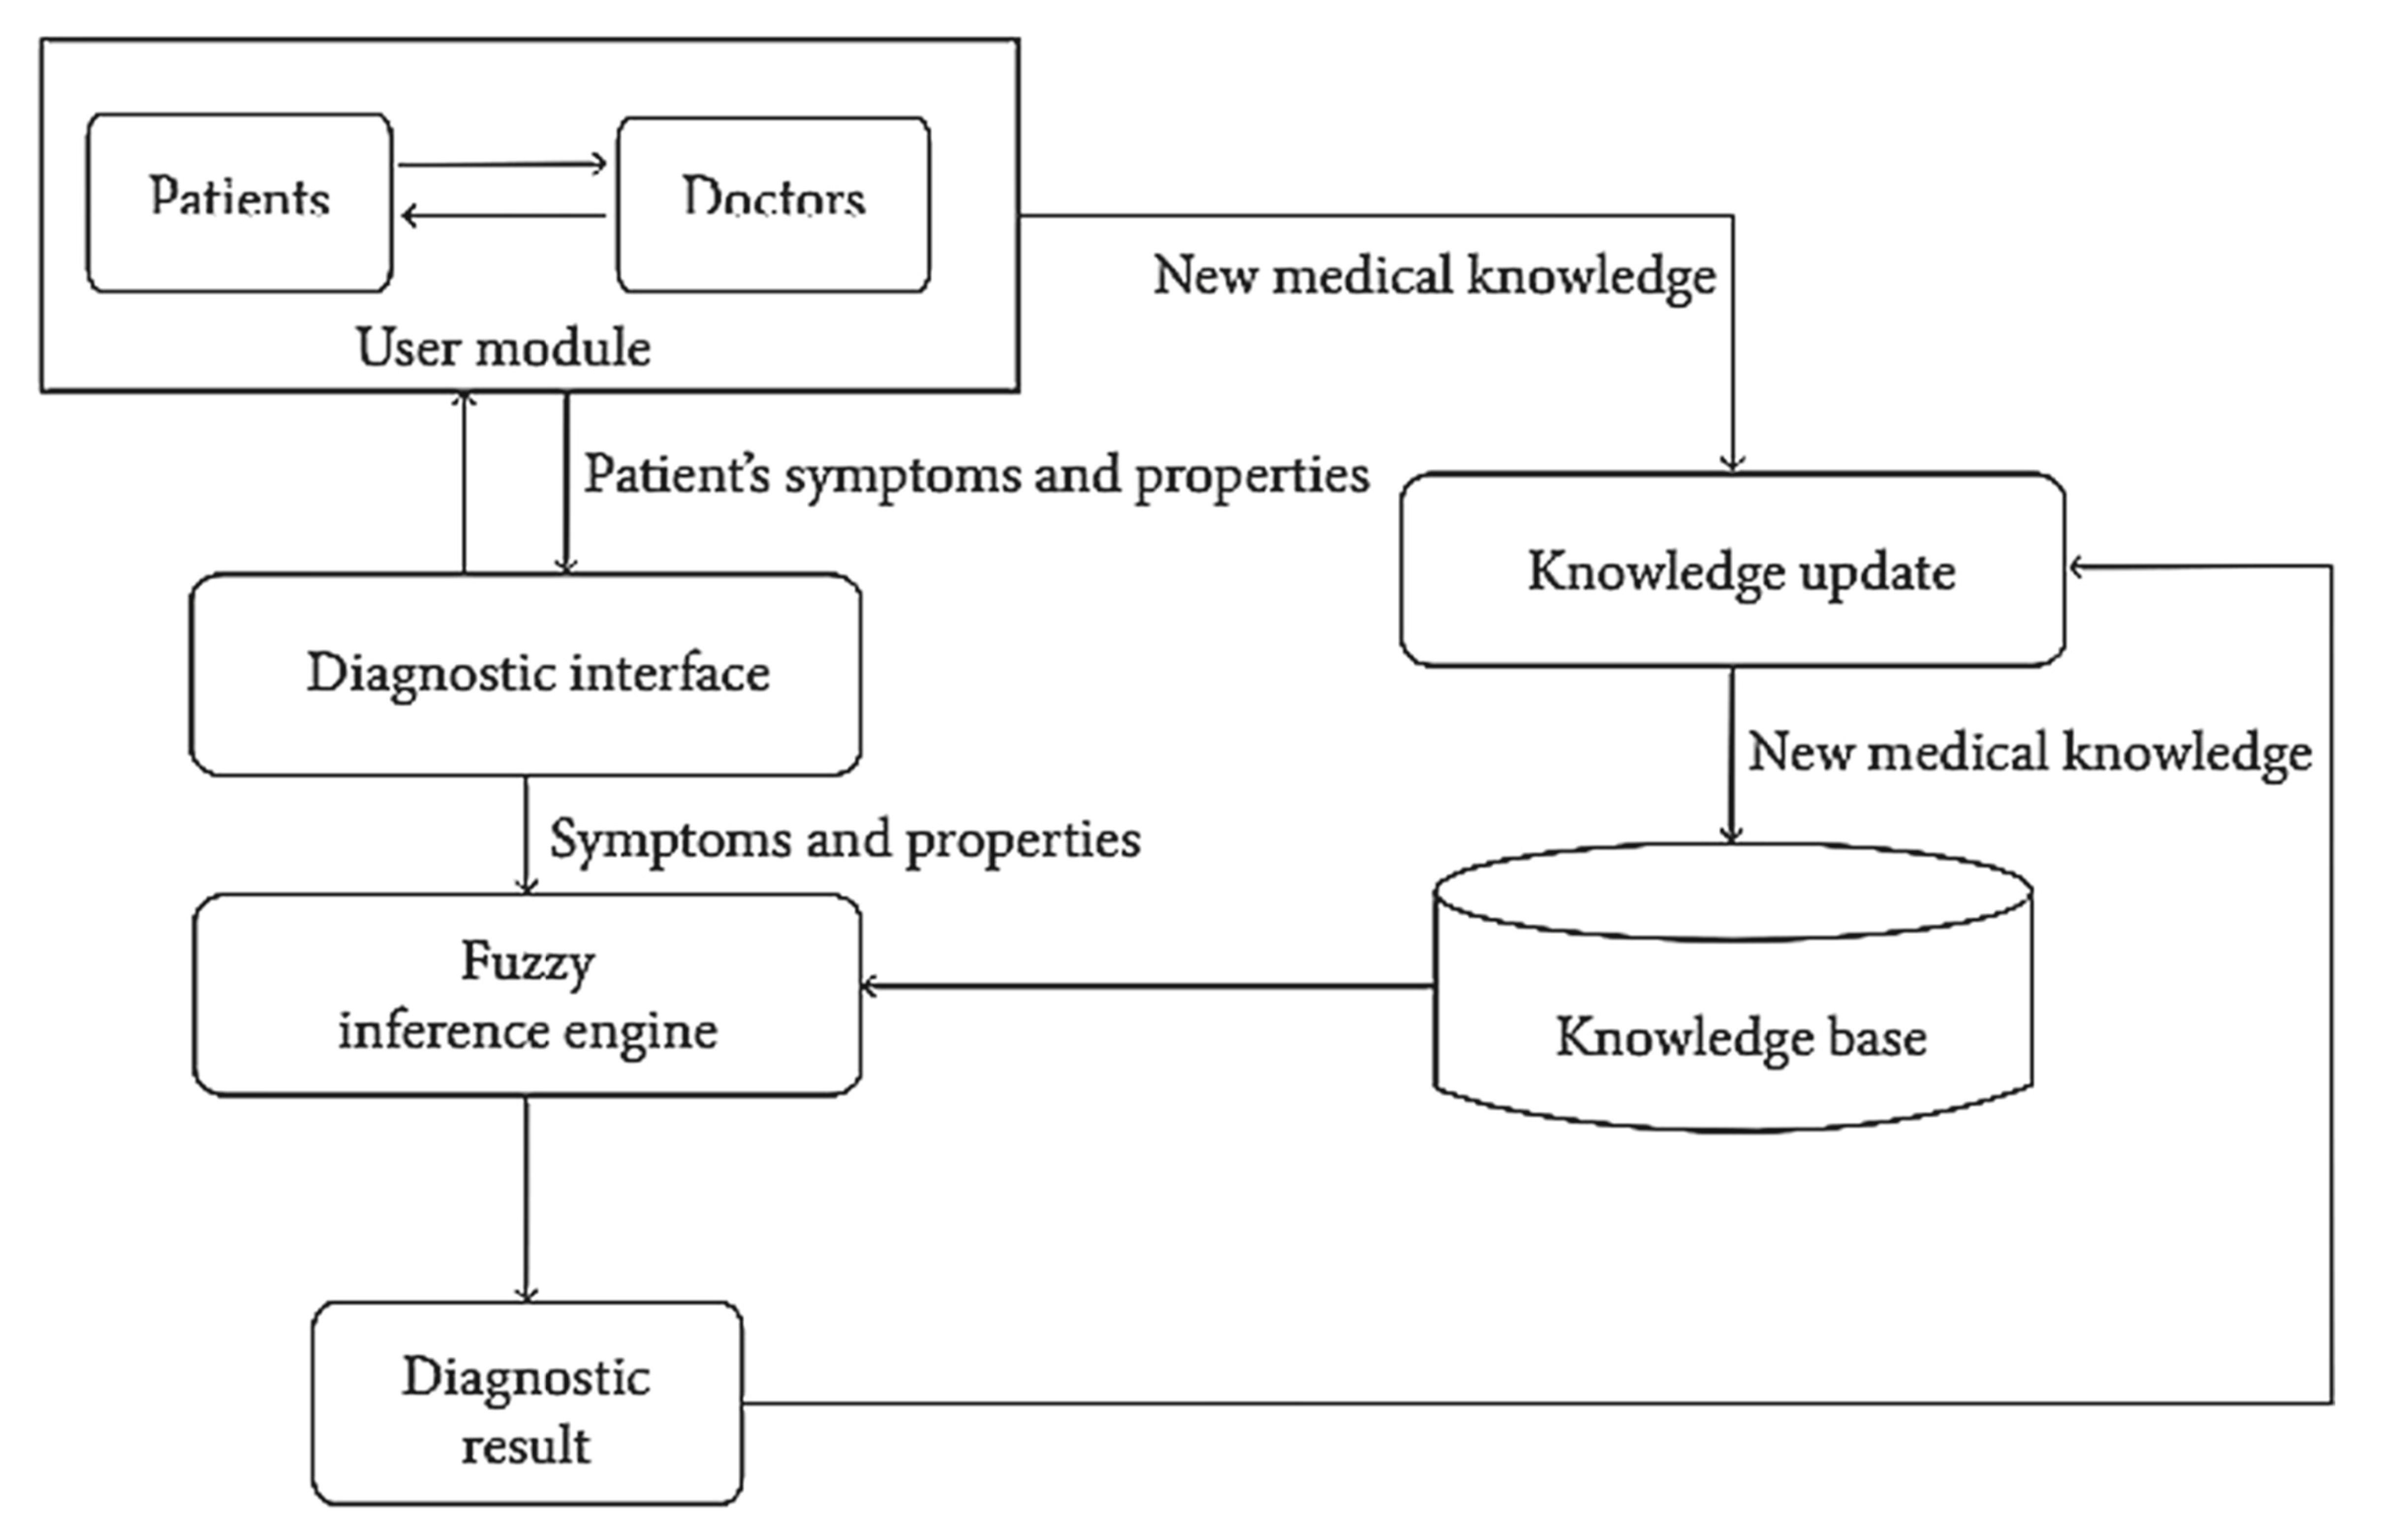
\includegraphics[width=0.6\textwidth]{2/1_antecedentes/Metodologia-9.png}
		\caption{Metodologia. Fuente: \cite{ApproachtoMedical}}
	\end{center}
\end{figure}
\vspace{-10mm}
\begin{enumerate}
	
	\item \textbf{Recolección y Preparación de Datos:}
		\subitem \textbf{Dataset de Síntomas:} Se recopiló un conjunto de datos de síntomas y enfermedades de diversas fuentes médicas confiables. Este dataset se utiliza para entrenar el modelo de aprendizaje automático.
	
		\subitem \textbf{Limpieza y Preprocesamiento de Datos:} Se eliminaron errores ortográficos y gramaticales de los datos recopilados para asegurar su calidad. Se utilizaron técnicas de tokenización y extracción de características para preparar los datos para el análisis.
	
	\item \textbf{Desarrollo del Modelo de Diagnóstico:}
		\subitem \textbf{Entrenamiento del Modelo:} Utilizando AWS Lex, se entrenó un modelo de lenguaje que puede analizar las consultas de los usuarios y generar diagnósticos basados en los síntomas proporcionados.
		
		\subitem \textbf{Integración con Servicios en la Nube:} AWS Lambda y Twilio se integraron para permitir la comunicación segura entre el chatbot y los usuarios a través de WhatsApp. Este sistema permite que el chatbot acceda a una base de datos de conocimiento médico y genere respuestas en tiempo real.
	
	\item \textbf{Implementación de Medidas de Seguridad:}
	
		\subitem \textbf{Protección de Datos:} Se implementaron sistemas de prevención de pérdida de datos y encriptación para proteger la información sensible de los usuarios. Twilio asegura que los datos solo sean accesibles por dispositivos autorizados y se sigue el principio de menor privilegio para el acceso a la información.
		
		\subitem \textbf{Auditorías y Cumplimiento:} AWS certifica que las medidas de seguridad cumplen con los requisitos legislativos, contractuales y regulatorios necesarios para manejar datos médicos sensibles.
	
	\item \textbf{Evaluación:}
		
		\subitem \textbf{Pruebas de Rendimiento:} Se realizaron pruebas exhaustivas para evaluar la precisión y relevancia de los diagnósticos generados por el chatbot. Se utilizó un enfoque de validación cruzada para asegurar la robustez del modelo.
		
\end{enumerate}

\subsubsection{Resultados obtenidos}
	DiagZone demostró ser efectivo en la provisión de diagnósticos médicos precisos y relevantes. En pruebas de rendimiento, el chatbot fue capaz de analizar los síntomas proporcionados por los usuarios y sugerir posibles enfermedades junto con medidas correctivas adecuadas. El sistema también pudo referir a los usuarios a médicos en caso de que los síntomas indicaran una condición más grave. La integración con WhatsApp a través de Twilio permitió una comunicación rápida y segura, mientras que el uso de AWS Lex garantizó respuestas precisas basadas en el análisis de datos de síntomas. Los usuarios reportaron una alta satisfacción con la facilidad de uso y la rapidez de las respuestas proporcionadas por el chatbot.

\begin{figure}[H]
	\begin{center}
		\includegraphics[width=0.6\textwidth]{2/1_antecedentes/Resultado-9.png}
		\caption{Chat Between User and Bot Salli. Fuente: \cite{ApproachtoMedical} }
	\end{center}
\end{figure}
\vspace{-10mm}

\subsection{A Medical ChatBot \citep*{MedicalChatBot}} 

\subsubsection{Planteamiento del Problema}
	El acceso a información médica precisa y oportuna es esencial para el bienestar de las personas, pero muchas veces los usuarios no cuentan con el conocimiento necesario sobre tratamientos o síntomas de enfermedades específicas. Además, las visitas al hospital para problemas menores pueden ser costosas y consumir mucho tiempo, y las consultas telefónicas pueden ser no siempre efectivas. Se presenta un chatbot médico que utiliza procesamiento de lenguaje natural (NLP) para proporcionar orientación sobre temas de salud de manera inmediata y accesible, sin la necesidad de visitas físicas al hospital. Este sistema no solo pretende ahorrar tiempo y reducir la carga sobre los servicios médicos, sino también ofrecer un recurso educativo para aquellos interesados en mejorar su conocimiento sobre salud y bienestar. 

\subsubsection{Fundamento Teórico}
El desarrollo del chatbot médico se fundamenta en varias teorías y tecnologías clave:

\begin{itemize}
	\item \textbf{Procesamiento de Lenguaje Natural (NLP):} El NLP permite a las máquinas comprender e interpretar el lenguaje humano, facilitando la interacción entre el usuario y el chatbot. Técnicas como el etiquetado de partes del discurso y el análisis semántico se utilizan para interpretar correctamente las consultas de los usuarios y generar respuestas adecuadas.
	
	\item \textbf{Algoritmo de Máquina de Vectores de Soporte (SVM):} El SVM permitira diferenciar entre diferentes clases basándose en los datos de entrenamiento. En el contexto del chatbot médico, se utiliza para predecir enfermedades. 
	
	\begin{figure}[H]
		\begin{center}
			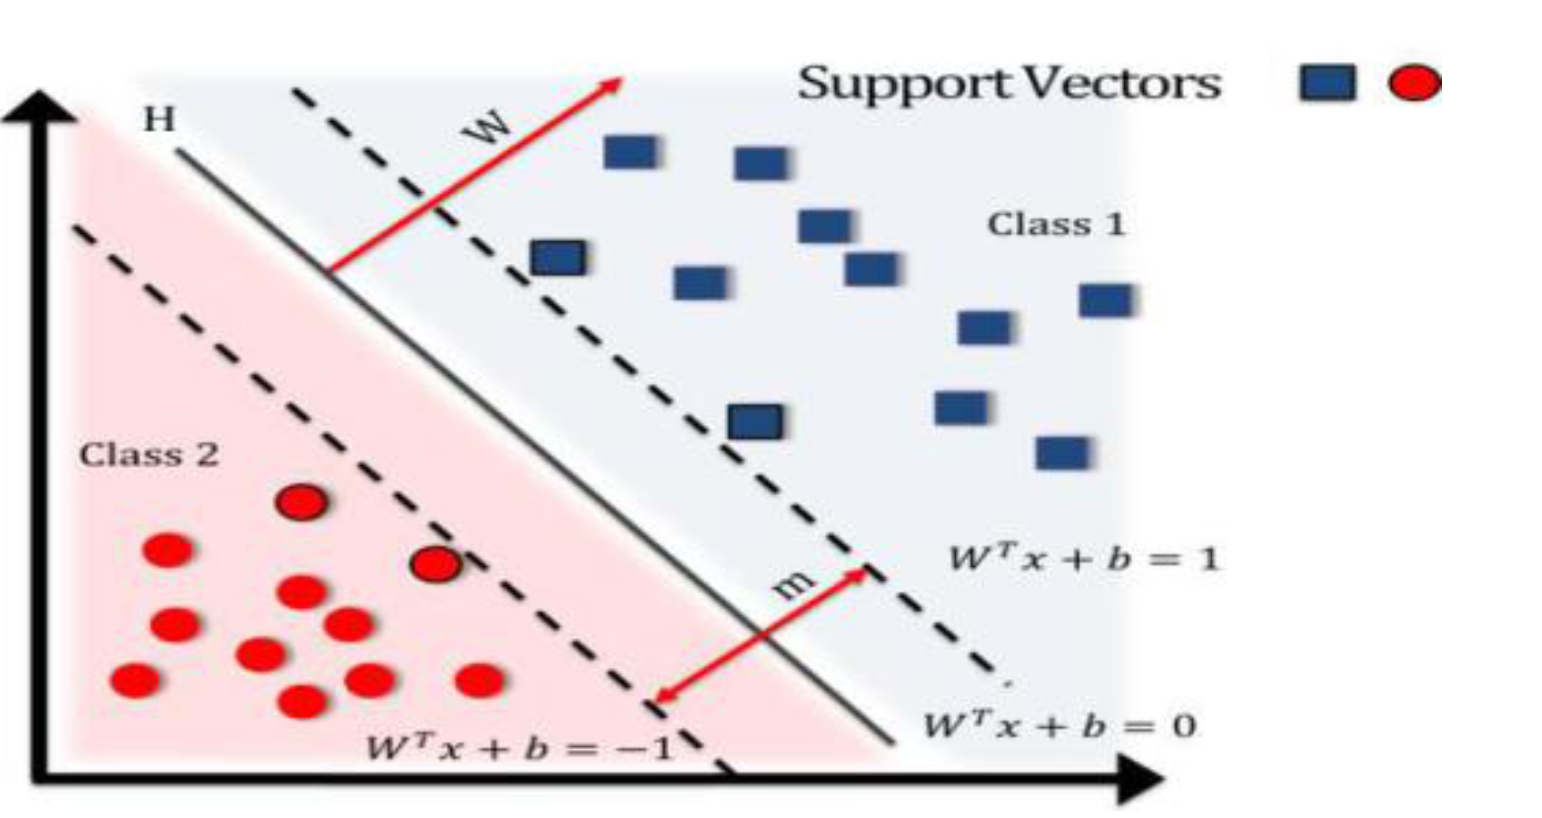
\includegraphics[width=0.6\textwidth]{2/1_antecedentes/SVM-10.png}
			\caption{Separando hiperplano por ecuación. Fuente: \cite{MedicalChatBot} }
		\end{center}
	\end{figure}
	\vspace{-10mm}
	\item \textbf{Similitud de Orden de Palabras:}La similitud de orden de palabras es importante para asegurar que el significado de las oraciones se mantenga coherente. Diferentes órdenes de palabras pueden alterar significativamente el significado de una oración.
	
	\item \textbf{Algoritmo de Stemming de Porter:} Este algoritmo se utiliza para reducir las palabras a su raíz o forma base, eliminando sufijos comunes. Esto ayuda a normalizar los datos textuales y mejora la precisión del análisis de NLP.
	
	\item \textbf{Interfaz de Usuario Gráfica (GUI):} Una GUI eficiente es crucial para facilitar la interacción entre el usuario y el chatbot, simulando una conversación humana.
	
	\item \textbf{APIs de Google:} Las APIs de Google para la conversión de voz a texto y reversa se utilizan para facilitar la comunicación verbal con el chatbot. Permite a usuarios interactuar con el sistema utilizando comandos de voz, mejorando la accesibilidad para personas con discapacidades visuales o dificultades para escribir.
\end{itemize}

\subsubsection{Metodología empleada por los autores}
	La metodología empleada incluye varias etapas clave:
	
	\begin{figure}[H]
		\begin{center}
			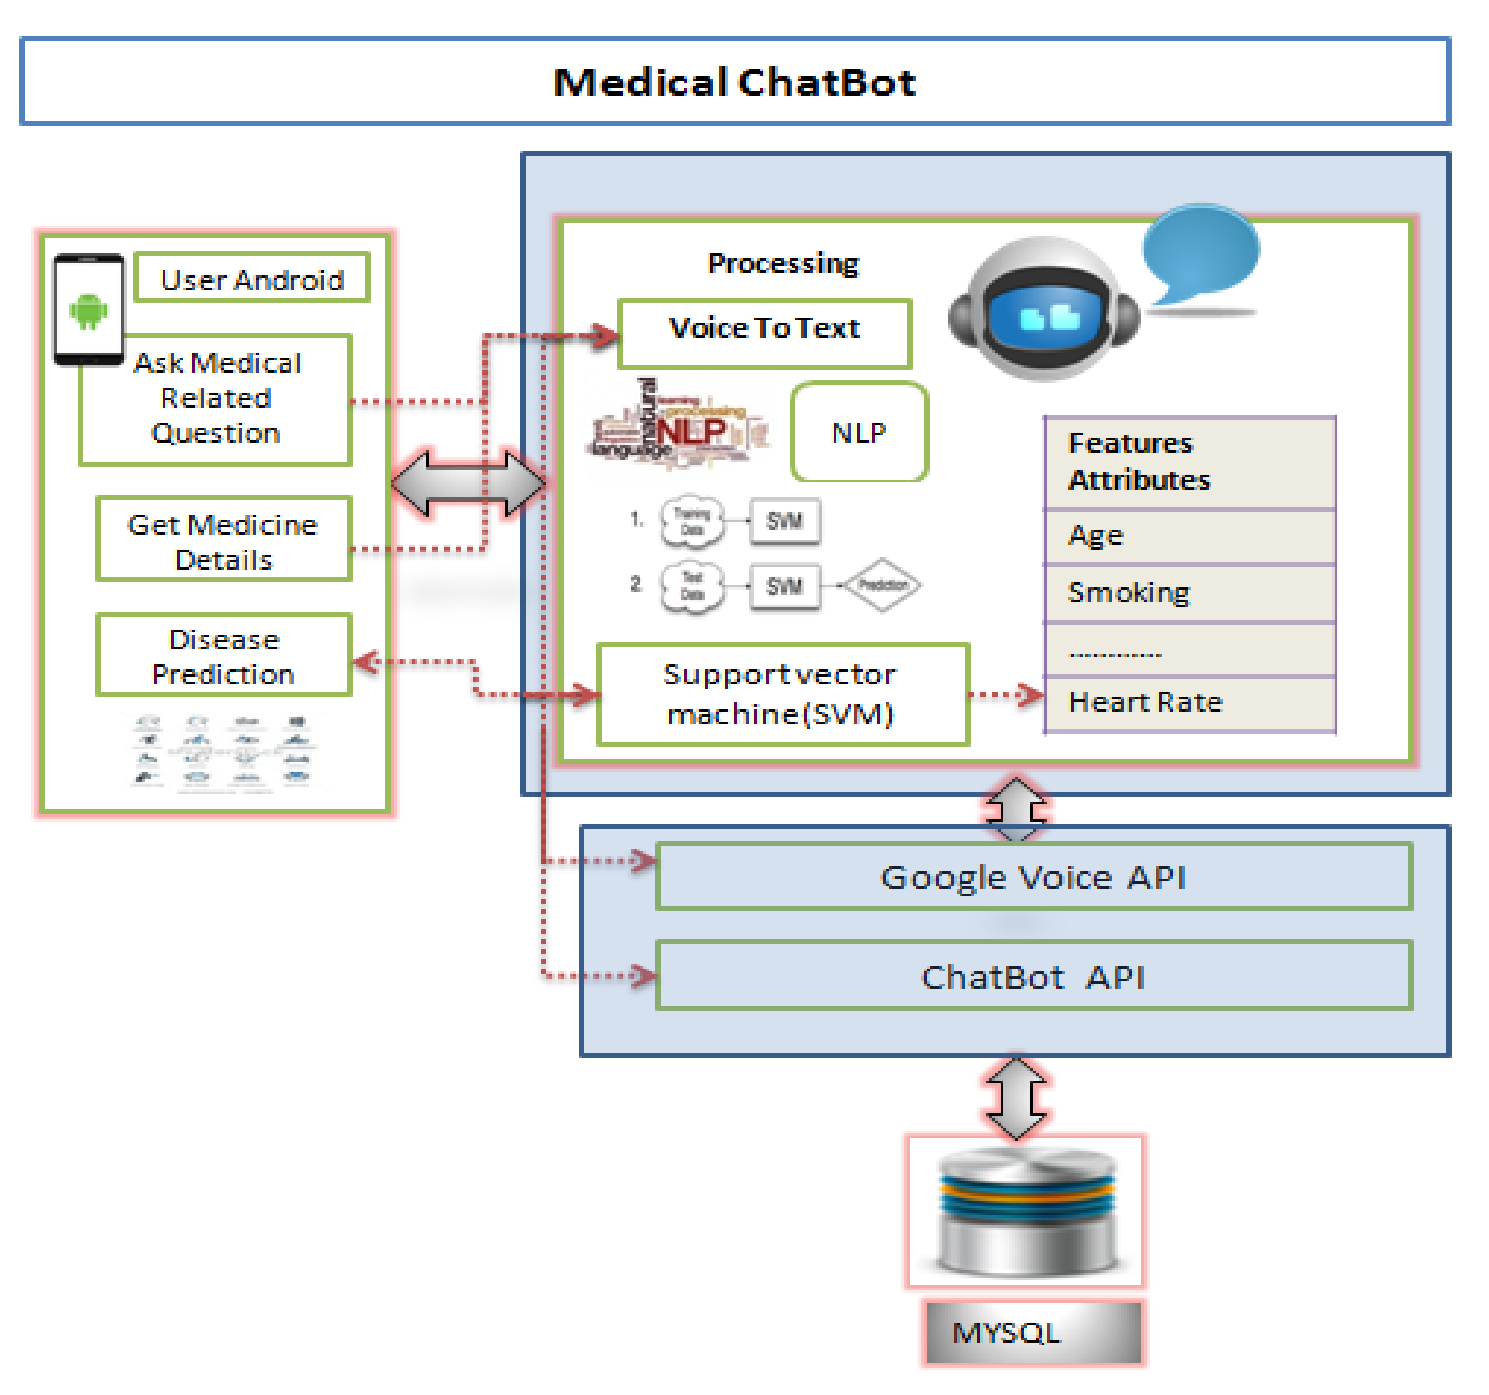
\includegraphics[width=0.6\textwidth]{2/1_antecedentes/Metodologia-10.png}
			\caption{Metodologia del Medical Chatbot. Fuente: \cite{MedicalChatBot}}
		\end{center}
	\end{figure}
\vspace{-10mm}
\begin{enumerate}
	
	\item \textbf{Recolección y Preparación de Datos:}
		\subitem \textbf{Dataset de Síntomas y Enfermedades:} Se recopiló un conjunto de datos de síntomas y enfermedades de diversas fuentes médicas confiables. Estos datos fueron limpiados y preprocesados para asegurar su calidad y relevancia.
		
		\subitem \textbf{Filtrado de Datos:}Se aplicaron técnicas de limpieza de datos para corregir errores ortográficos y gramaticales, así como para eliminar cualquier ruido o datos irrelevantes.
	
	\item \textbf{Desarrollo del Modelo de Diagnóstico:}
		\subitem \textbf{Entrenamiento del Modelo SVM:} Se entrenó un modelo de SVM para clasificar y predecir enfermedades basándose en los síntomas proporcionados por los usuarios. Este modelo fue ajustado para maximizar la precisión y minimizar los errores de clasificación.
		
		\subitem \textbf{Implementación de NLP:} Se integraron técnicas de NLP para analizar y comprender las consultas de los usuarios. Esto incluye el uso de algoritmos de stemming, etiquetado de partes del discurso y análisis semántico para interpretar correctamente las entradas de texto.
	
	\item \textbf{Desarrollo de la Interfaz de Usuario:}
	
		\subitem \textbf{Diseño de la GUI:} Se diseñó una interfaz gráfica intuitiva y fácil de usar para facilitar la interacción entre los usuarios y el chatbot. La GUI incluye funciones para la entrada de texto y voz, así como para la visualización de respuestas.
		
		\subitem \textbf{Integración con APIs de Google:} Las APIs de Google para la conversión de voz a texto y de texto a voz se integraron en el sistema para permitir la comunicación verbal con el chatbot.
	
	\item \textbf{Implementación de la Similitud de Orden de Palabras:}
	
		\subitem \textbf{Cálculo de la Similitud:} Se implementaron técnicas para calcular la similitud de orden de palabras entre las consultas de los usuarios y las respuestas almacenadas en la base de datos.
	
		\subitem \textbf{Optimización del Umbral:} Se ajustó el umbral de similitud para equilibrar la precisión y la relevancia de las respuestas generadas, asegurando que el chatbot proporcione respuestas útiles y coherentes.
			
	\item \textbf{Evaluación:}
	
		\subitem \textbf{Pruebas de Rendimiento:} Se realizaron pruebas exhaustivas para evaluar la precisión y relevancia de los diagnósticos generados por el chatbot. Se utilizó un enfoque de validación cruzada para asegurar la robustez del modelo y evitar el sobreajuste. 
	
\end{enumerate}

\subsubsection{Resultados obtenidos}

	El chatbot médico demostró ser efectivo en la provisión de diagnósticos médicos precisos y relevantes. En las pruebas de rendimiento, el modelo de SVM logró una precisión del 94\%, superando significativamente a los métodos K-nearest neighbors y Naive Bayes. El uso de técnicas de NLP permitió al chatbot interpretar correctamente las consultas de los usuarios y generar respuestas útiles basadas en los datos de síntomas y enfermedades. La integración con APIs de Google facilitó la comunicación verbal con el chatbot, mejorando la accesibilidad para una mayor variedad de usuarios. Los usuarios expresaron una gran satisfacción con la facilidad y precisión del diagnóstico proporcionado por el chatbot.
	
	\begin{figure}[H]
		\begin{center}
			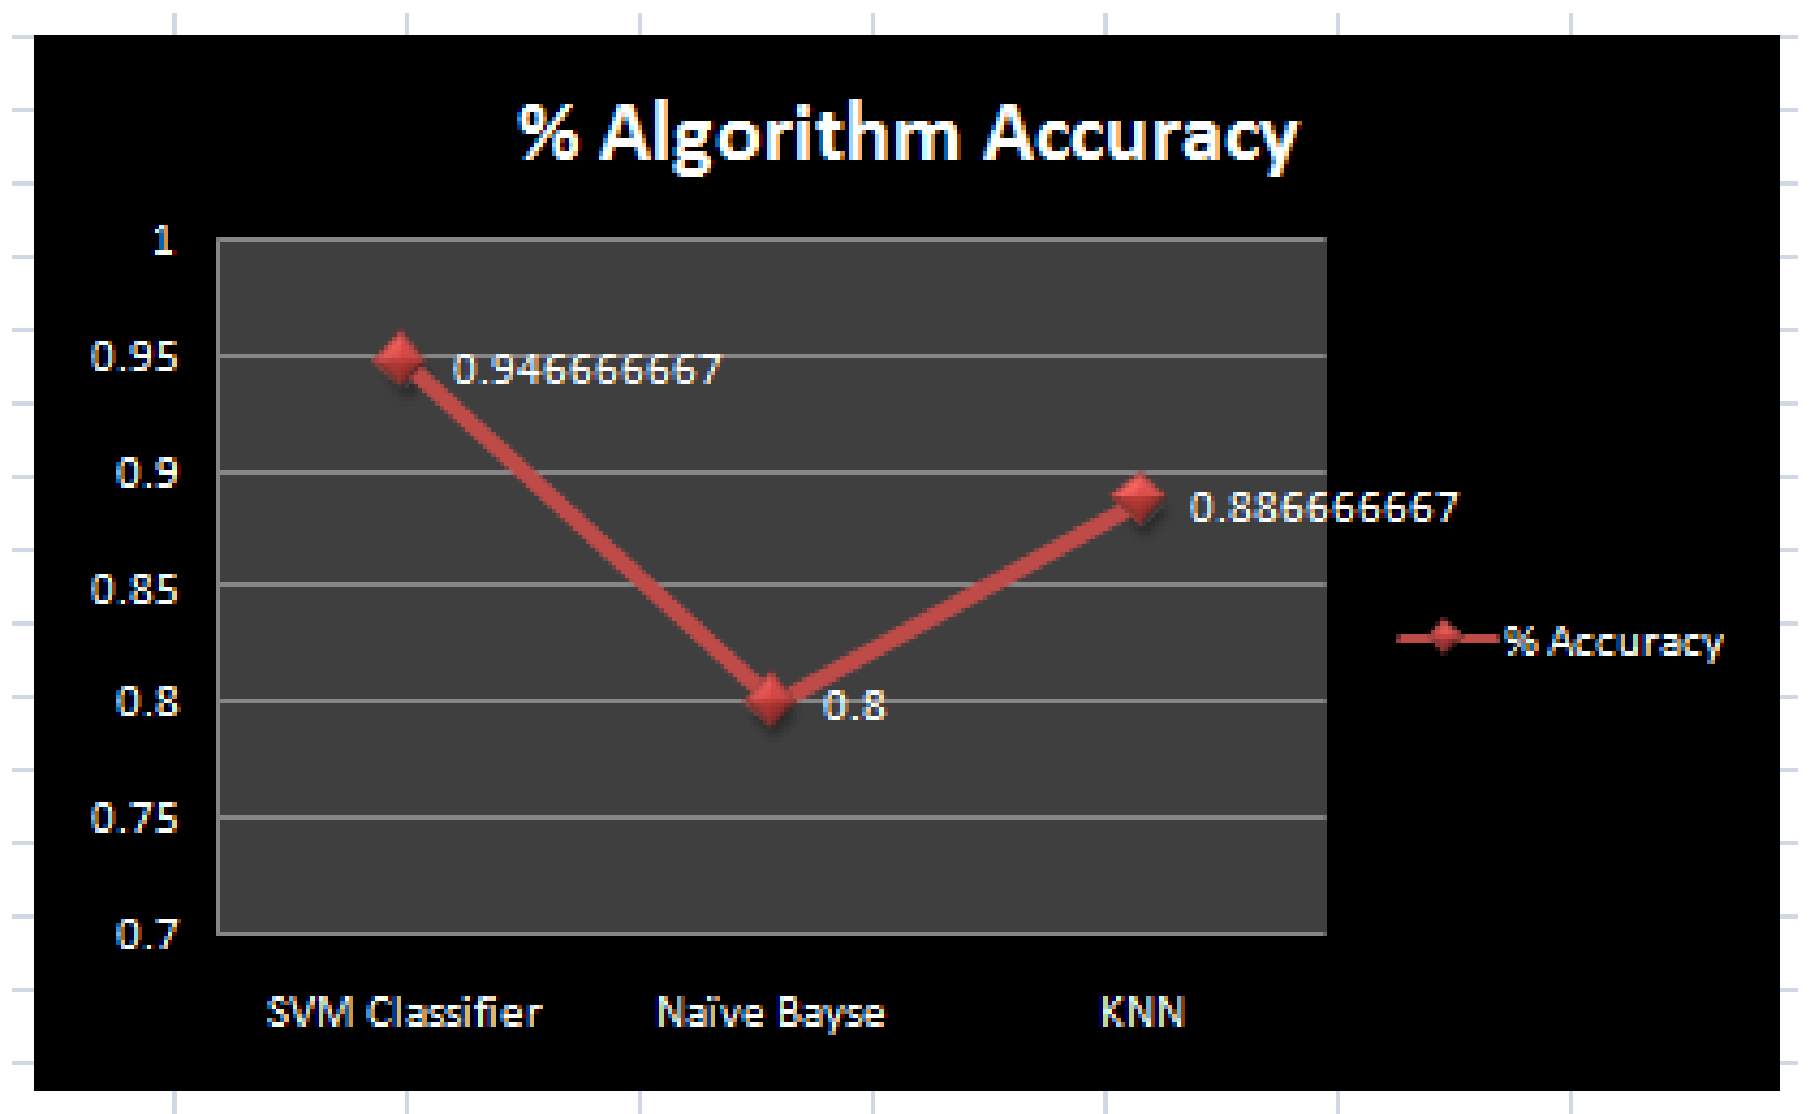
\includegraphics[width=0.6\textwidth]{2/1_antecedentes/Resultado2-10.png}
			\caption{Algoritmo de Exactitud despues de la comparación de diferentes métodos. Fuente: \cite{MedicalChatBot} }
		\end{center}
	\end{figure}
	
\vspace{-10mm}